\documentclass{report}

% Font
\usepackage[T1]{fontenc}
% https://es.overleaf.com/learn/latex/Font_sizes%2C_families%2C_and_styles
\renewcommand{\familydefault}{\sfdefault}

% Saltear indentación en los párrafos
% https://tex.stackexchange.com/questions/14375/how-to-disable-automatic-indentation-on-new-paragraphs
\usepackage{parskip}

% Matemática
\usepackage{amsmath}    % símbolos matemáticos
\usepackage{amssymb}    % símbolos matemáticos
\usepackage{amsthm}     % teoremas
\usepackage{amsfonts}   % \mathbb
\usepackage{bm}         % bold math (https://ctan.org/pkg/bm)
\usepackage{abraces}    % \aunderbrace y \aoverbrace
\usepackage{mathtools}  % \mathclap

% Para hacer derivaciones y eso
% https://personal.utdallas.edu/~hamlen/trfrac.pdf
\usepackage{tfrac}

% Figuras
\usepackage{tikz}                   % gráficos
\usepackage{float}                  % [H]
\usepackage{xcolor}                 % colores https://es.overleaf.com/learn/latex/Using_colours_in_LaTeX

\usepackage{framed}     % textbars

\usepackage{graphicx} % Imagenes
\graphicspath{img/}

% Texto
\usepackage[shortlabels]{enumitem}  % enumerate con letras

% Referencias
\usepackage[colorlinks=true]{hyperref}

% https://tex.stackexchange.com/questions/121865/nameref-how-to-display-section-name-and-its-number
\newcommand*{\fullref}[1]{\hyperref[{#1}]{\autoref*{#1} \nameref*{#1}}}

% Programas
% https://tex.stackexchange.com/questions/116595/highlighting-haskell-listings-in-large-tex-document
% https://leportella.com/minted-vscode/
% https://tex.stackexchange.com/questions/367332/minted-error-undefined-control-sequence-pyg-with-texmaker
\usepackage[cache=false]{minted}     % código

% https://tex.stackexchange.com/questions/260566/how-to-reliably-switch-the-highlighting-color-with-soul
\usepackage{soul}
\DeclareRobustCommand{\hlcyan}[1]{{\sethlcolor{cyan}\hl{#1}}}


\usetikzlibrary{arrows,positioning,automata,shadows,fit,shapes}

% Teoremas, corolarios, etc.
% https://www.overleaf.com/learn/latex/theorems_and_proofs
\theoremstyle{definition} % Para que no salga en italicas

\newtheorem{theorem}{Teorema}[chapter]
\newtheorem*{theorem*}{Teorema}

\newtheorem{lemma}{Lema}[chapter]
\newtheorem*{lemma*}{Lema}

\newtheorem{proposition}{Prop.}[chapter]
\newtheorem*{proposition*}{Prop}

\newtheorem{definition}{Def.}[chapter]
\newtheorem*{definition*}{Def}

\newtheorem{observation}{Obs.}[chapter]
\newtheorem*{observation*}{Obs}

\newtheorem{example}{Ejemplo}[chapter]
\newtheorem*{example*}{Ejemplo}

% https://tex.stackexchange.com/questions/118173/how-to-write-ceil-and-floor-in-latex
\DeclarePairedDelimiter\ceil{\lceil}{\rceil}
\DeclarePairedDelimiter\floor{\lfloor}{\rfloor}

% Comandos de PLP
%\newcommand{\sigmatsequence}{\overset{\rightarrow}{\sigma}}
%\newcommand{\tautsequence}{\overset{\rightarrow}{\tau}}

% Entornos
\newenvironment{nota}[1]
    {\begin{leftbar}\textbf{#1}}
    {\end{leftbar}}

% https://tex.stackexchange.com/questions/42619/x-mark-to-match-checkmark/42620
\usepackage{pifont} % http://ctan.org/pkg/pifont
\newcommand{\cmark}{\ding{51}}
\newcommand{\xmark}{\ding{55}}

% Texto
\newcommand{\todo}[1]{{\textcolor{red}{\textbf{#1}}}}

% Mate general
\newcommand{\eqdef}{\overset{\text{def}}{=}}
\newcommand{\aeq}{=_\alpha}
\newcommand{\naeq}{\neq_\alpha}

% Calculo lambda
\newcommand{\extendTypesWith}[1]{\sigma ::= \dots \mid #1}
\newcommand{\lambdab}{\lambda^b}

\newcommand{\tfunc}[2]{#1 \to #2}
\newcommand{\ifte}[3]{\ \text{if } #1 \text{ then } #2 \text{ else } #3}
\newcommand{\abs}[3]{\lambda #1 : #2 . #3}
\newcommand{\app}[2]{#1 \ #2} % aplicación
\newcommand{\sust}[2]{#1 \{ #2 \}}
\newcommand{\sustOne}[3]{#1 \{ #2 \leftarrow #3 \}}

\newcommand{\uabs}[2]{\lambda #1 . #2} % untyped

\newcommand{\tipa}[3]{#1 \rhd #2 : #3} % \vartriangleright
\newcommand{\tienetipo}[3]{#1 : #2 \in #3}
\newcommand{\Gtipa}[2]{\tipa{\Gamma}{#1}{#2}}
\newcommand{\GStipa}[2]{\tipa{\Gamma|\Sigma}{#1}{#2}}
\newcommand{\compat}[2]{#1 \rhd #2} % compatibilidad
\newcommand{\GSCompat}[1]{\compat{\Gamma|\Sigma}{#1}} % compatibilidad

\newcommand{\fv}[1]{FV(#1)}

% Lambda bn
\newcommand{\lambdabn}{\lambda^{bn}}
\newcommand{\suc}[1]{succ(#1)}
\newcommand{\pred}[1]{pred(#1)}
\newcommand{\iszero}[1]{iszero(#1)}
\newcommand{\num}[1]{\underbar{#1}} % abreviación de suc^#1(0)

% Lambda reg
\newcommand{\lambdareg}{\lambda^{\dots r}}
\newcommand{\reg}[1]{\{\ #1\ \}}
\newcommand{\proj}[2]{#1 . #2}

\newcommand{\treg}[1]{\{ #1 \}}

\newcommand{\iesimo}[1]{#1_i^{\ \ i \in 1..n}}

% Lambda bnu
\newcommand{\lambdabnu}{\lambda^{bnu}}
\newcommand{\seq}[2]{#1;#2}

% Lambda let
\newcommand{\lambdalet}{\lambda^{\dots let}}
\newcommand{\letin}[4]{\text{let } #1 : #2 = #3 \text{ in } #4}
\newcommand{\uletin}[3]{\text{let } #1 = #2 \text{ in } #3} % untyped
\newcommand{\alloc}[1]{\text{ref } #1}
\newcommand{\dealloc}[1]{!#1}
\newcommand{\assign}[2]{#1 := #2}

\newcommand{\unit}{unit}
\newcommand{\tunit}{Unit}

\newcommand{\tref}[1]{\text{Ref } #1}

\newcommand{\dom}[1]{Dom(#1)}

\newcommand{\store}[3]{#1 [#2 \mapsto #3]}
\newcommand{\estore}[3]{#1 \oplus (#2 \mapsto #3)}
\newcommand{\mustore}[2]{\store{\mu}{#1}{#2}}
\newcommand{\emustore}[2]{\estore{\mu}{#1}{#2}}

\newcommand{\mematSet}[3]{#1(#2) = #3}
\newcommand{\memat}[2]{#1(#2)}

\newcommand{\sreduce}[4]{\reduce{#1\mid#2}{#3\mid#4}}
\newcommand{\sreduceToPrime}[2]{\sreduce{#1}{#2}{#1'}{#2'}}

\newcommand{\sreducesTo}[5]{#1\mid#2 \reducesTo{#3} #4\mid#5}
\newcommand{\expstore}[2]{#1 \mid #2}

% Recursión
\newcommand{\fix}[1]{\text{fix } #1}
\newcommand{\letrec}[4]{\text{letrec } #1 : #2 = #3 \text{ in } #4}

% Reducciones
\newcommand{\reduces}{\to}
\newcommand{\reducesTo}[1]{\reduces_\text{(#1)}}
\newcommand{\reduce}[2]{#1 \reduces #2}
\newcommand{\reduceToPrime}[1]{\reduce{#1}{#1'}}
\newcommand{\doesntReduce}[2]{#1 \not\reduces #2}

\newcommand{\reduceManyTo}{\twoheadrightarrow}
\newcommand{\reduceMany}[2]{#1 \reduceManyTo #2}

\newcommand{\deriv}[3]{\trfrac[(#1)]{#2}{#3}}
\newcommand{\derivok}[1]{\trfrac[]{\checkmark}{#1}}
\newcommand{\ederiv}[2]{\trfrac{#1}{#2}} % empty deriv

% Para indicar que algo se conv en valor
\newcommand{\changed}[1]{\textcolor{red}{#1}}
\newcommand{\select}[1]{\textcolor{blue}{#1}}

\newcommand{\evalsto}{\leadsto}

% Inferencia
\newcommand{\untypedTerms}{\Lambda}
\newcommand{\typedTerms}{\Lambda_\tau}
\newcommand{\typeVars}{\mathcal{V}}
\newcommand{\types}{\mathcal{T}}
\newcommand{\erase}[1]{\text{Erase}(#1)}

\newcommand{\tsust}[1]{S#1} % apply type sust
\newcommand{\sustfor}[2]{#1/#2} % type sust

\newcommand{\GTipaInst}[2]{\tipa{\Gamma'}{#1'}{#2'}} % instancia

\newcommand{\infer}[1]{\mathbb{W}(#1)}

\newcommand{\tcontextOne}[2]{\{ #1 : #2 \}} % type context
\newcommand{\etipa}[2]{\tipa{\emptyset}{#1}{#2}} % emptyset tipa

\newcommand{\comp}[2]{#1 \circ #2}
\newcommand{\unify}[2]{#1 \doteq #2}

\newcommand{\unifySetD}{\{
    \unify{\sigma_1}{\sigma_1'},
    \dots,
    \unify{\sigma_n}{\sigma_n'} 
\}}

%% Unificación
\newcommand{\simpSust}[1]{\mapsto_{#1}}
\newcommand{\simp}{\mapsto}

\newcommand{\asimpSust}[2]{\mapsto_{#2}^{#1}} % annotated
\newcommand{\asimp}[1]{\mapsto^{#1}}

\newcommand{\mgu}[2]{\text{MGU}(\{ \unify{#1}{#2} \})}

% Resolución
\newcommand{\resol}[2]{\frac{#1}{#2}}

% Subtipado
\newcommand{\subt}[2]{#1 <: #2}

\newcommand{\ligada}[1]{\underbrace{#1}_{\text{ligada}}}
\newcommand{\libre}[1]{\underbrace{#1}_{\text{libre}}}

\newcommand{\tsource}[1]{\text{Source } #1}
\newcommand{\tsink}[1]{\text{Sink } #1}

\author{Manuel Panichelli}
\title{Notas para final de PLP}

\begin{document}

\maketitle

\tableofcontents

\chapter{Paradigma funcional}

\section{Haskell}

\begin{definition}[Paradigma]
    Un \textbf{paradigma} es una forma de pensamiento.
\end{definition}

\begin{definition}[Lenguaje de programación]
    Un \textbf{lenguaje de programación} es el lenguaje que usamos para
    comunicar lo que queremos que haga una computadora.

    Usamos un lenguaje para describir los computos que lleva a cabo la
    computadora.
    
    Es \textbf{computacionalmente completo} si puede expresar todas las
    funciones computables. Hay DSLs (\textit{domain specific languages}) que no
    pueden expresar todo lo computable.
\end{definition}

\begin{definition}[Paradigma de lenguaje de programación]
    Lo entendemos como un \textit{estilo} de programación, que tiene que ver con
    los estilos de las soluciones. Está vinculado con lo que es para uno un
    modelo de cómputo.

    Lo que vemos antes de la materia es el imperativo: a partir de un estado
    inicial llegar a un estado final. Programamos con secuencias de
    instrucciones para cambiar el estado.
\end{definition}

\subsection{Programación funcional}

Definiciones:

\begin{itemize}
    \item \textbf{Programa y modelo de cómputo}: Programar es definir
    funciones, y ejecutar es evaluar expresiones.
    \item \textbf{Programa}: Es un conjunto de ecuaciones. Por ej.
    \texttt{doble x = x + x}
    \item \textbf{Expresiones}: El significado de una expresión es su valor
    (si es que está definido). El valor de una expresión depende solo del
    valor de sus sub-expresiones. Evaluar o reducir una expresion es obtener
    su valor (por ej. \texttt{doble 2 $\leadsto$ 4})
    No toda expresion denota un valor, por ejemplo \texttt{doble true}.
    \item \textbf{Tipos}: El universo de valores está particionado en
    colecciones denominadas \textit{tipos}, que tienen operaciones asociadas.
\end{itemize}

Haskell es \textbf{fuertemente tipado}. Toda expresion bien formada tiene un
tipo, que depende del tipo de sus subexpresiones. Si no puede asignarse un tipo
a una expresión, no se la considera bien formada.

\begin{minted}{haskell}
1           :: Int
'a'         :: Char
1.2         :: Float
True        :: Bool
[1, 2, 3]   :: [Int]
(1, True)   :: (Int, Bool)
succ        :: Int -> Int
\end{minted}

Definiciones de funciones:

\begin{minted}{haskell}
-- Definición
doble :: Int -> Int
doble x = x + x

-- Guardas
signo :: Int -> Bool
signo n | n >= 0    = True
        | otherwise = False

-- Definiciones locales
f (x, y) = g x + y
    where g z = z + 2

-- Expresiones lambda
\x -> x + 1
\end{minted}

\textbf{Tipos polimórficos}

\begin{minted}[]{haskell}
    id x = x
    id :: a -> a
    -- x es de tipo a, que eventualmente se va a instanciar a algún tipo
\end{minted}

\textbf{Clases de tipos}: Son como interfaces, que definen un conjunto de
operaciones.

\begin{minted}[]{haskell}
    maximo :: Ord a => a -> a -> a
    maximo x y | x > y = x
    maximo _ y = y
    -- Ord: (<), (<=), (>=), (>), max, min, compare
\end{minted}

\textbf{Tipos algebráicos}

\begin{minted}[]{haskell}
    data Figura = Circulo Float | Rectangulo Float Float
    deriving Eq -- deriva la igualdad nativa

    -- (Circulo 1) == (Circulo 1)
\end{minted}

Estas cosas nos permiten hacer funciones genéricas.

\textbf{Funciones de alto orden}: las funciones son first class citizens, se
pueden pasar como parámetro.

\subsection{Currificación}

Es un mecanismo que permite reemplazar argumentos estructurados por una
secuencia de argumentos "simples". Ventajas:

\begin{itemize}
    \item Evaluación parcial: \texttt{succ = suma 1}
    \item Evita escribir paréntesis (asumiendo que la aplicación asocia a
    izquierda). \texttt{suma 1 2 = ((suma 1) 2)}
\end{itemize}

\textbf{curry y uncurry}

En criollo: una equivalencia entre una func con muchos parametros (una tupla) y
una funcion equivalente que va tomando de a uno y devuelve funciones.

\begin{minted}[]{haskell}
    curry :: ((a, b) -> c) -> (a -> (b -> c))
    curry f a b = f (a, b)

    suma x y = x + y
    suma' :: (Int, Int) -> Int
    suma' (x, y) = x + y

    curry suma' 1 2 = suma' (1, 2)
    curry suma' :: (Int -> (Int -> Int))

    uncurry :: (a -> b -> c) -> ((a -> b) -> c)
    uncurry f (a, b) = f a b
\end{minted}

\subsection{Pattern matching}

Una forma copada de definir funciones. Es un mecanismo para comparar un valor
con un patrón. Si la comparación tiene éxito se puede deconstruir un valor en
sus partes.

\begin{minted}[]{haskell}
    data Figura = Circulo Float | Rectangulo Float Float

    area :: Figura -> Float
    area (Circulo radio) = pi * radio ^ 2
    area (Rectangulo l1 l2) = l1 * l2
\end{minted}

El patrón está formado por el constructor y las variables. Los casos se evalúan
en el orden en el que están escritos.

\begin{minted}[]{haskell}
    esCuadrado :: Figura -> Bool
    -- No vale esto?
    -- esCuadrado (Rectangulo x y) = (x == y)
    esCuadrado (Rectangulo x y) | (x==y) = True
    esCuadrado _ = False
\end{minted}

También se pueden definir funciones parciales (que no estén definidas para todo
el dominio).

\subsection{Tipos recursivos}
La definición de un tipo puede tener uno o más parámetros del tipo

\begin{minted}[]{haskell}
    data Natural = Zero | Succ Natural

    Zero :: Natural                     -- 0
    succ Zero :: Natural                -- 1
    succ (succ (succ Zero)) :: Natural  -- 2

    dameNumero :: Natural -> Int
    dameNumero Zero = 0
    dameNumero (Succ n) = dameNumero n + 1
\end{minted}

\subsection{Listas}

Tipo algebráico paramétrico recursivo con dos constructores:

\begin{minted}[]{haskell}
    [] :: [a]               -- lista vacia
    (:) :: a -> [a] -> [a]  -- constructor infijo

    -- Ejemplo
    --   1 : [2, 3] = [1, 2, 3]
\end{minted}

Pattern matching

\begin{minted}[]{haskell}
    vacia :: [a] -> Bool
    vacia [] = True
    vacia _ = False

    long :: [a] -> Int
    long [] = 0
    long x:xs = 1 + long xs
\end{minted}

\subsection{No terminación y orden de evaluación}

\begin{minted}[]{haskell}
    -- No terminación
    inf1 :: [Int]
    inf1 = 1 : inf1

    -- Evaluación no estricta
    const :: a -> b -> a
    const x y = x

    -- const 42 inf1 -> 42 (pero depende del mecanismo de reducción del
    -- lenguaje)
\end{minted}

\subsection{Evaluación lazy}

el modelo de cómputo de haskell es la \textbf{reducción}. Se reemplaza un
\textit{redex} por otro usando las ecuaciones orientadas. Un redex (reducible
expression) es una sub-expresión que no está en forma normal (irreducible).

Un redex debe ser una \textbf{instancia} del lado izquierdo de alguna ecuación y
será reemplazado por el lado derecho con las variables correspondientes ligadas.
El resto de la expresión no cambia.

Haskell hace esto hasta llegar a una forma normal, un valor irreducible.

\texttt{const x y = x}. \texttt{const x y} es un redex, y lo reduzco a
\texttt{x}.

Y cómo selecciono una redex? \textbf{Orden normal} (lazy). Se selecciona el
redex más externo para el que se pueda conocer que ecuación del programa
utilizar. En general, primero las funciones más externas y luego los argumentos,
solo de ser necesarios.

Modo aplicativo: reduce primero todos los argumentos. Se hace en otros lenguajes
como c.

\subsection{Esquemas de recursion}

Formas de recursion comunes que uno puede aprovechar usando funciones de alto
orden.

\subsubsection{Map}

\begin{minted}[]{haskell}
-- tal que dobleL xs es la lista que contiene el doble de cada elemento en xs
dobleL :: [Float] -> [Float]
dobleL [] = []
dobleL (x:xs) = 2*x : dobleL xs

-- tal que la lista esParL xs indica si el correspondiente elemento en xs es par
-- o no
esParL :: [Int] -> [Bool] 
esParL [] = []
esParL (x:xs) = (even x) : esParL xs

-- tal que longL xs es la lista que contiene las longitudes de las listas en xs
longL :: [[a]] -> [Int]
longL [] = []
longL (x:xs) = (length x) : longL xs

-- esquema recursivo de map:
map :: (a -> b) -> [a] -> [b]
map _ [] = []
map g (x:xs) = g x : map g xs

-- Con eso, se pueden reescribir como
dobleL = map ((*) 2)
esParL = map even
longL = map length
\end{minted}

\subsubsection{Filter}

\begin{minted}{haskell}
-- tal que negativos xs contiene los elementos negativos de xs
negativos :: [Float] -> [Float]
negativos [] = []
negativos (x:xs)
    | x < 0 = x : (negativos xs)
    | otherwise = negativos xs

-- tal que la lista noVacias xs contiene las listas no vacias de xs
noVacias :: [[a]] -> [[a]]
noVacias [] = []
noVacias (l:ls)
    | (length l > 0) = l : (noVacias ls)
    | otherwise = noVacias ls

-- esquema recursivo:
filter :: (a -> Bool) -> [a] -> [a]
filter _ [] = []
filter p (x:xs) = if (p x) then x : (filter p xs)
                  else (filter p xs)

-- luego quedan
negativos = filter (\x -> x < 0)
noVacias = filter (\l -> length l != 0)
noVacias = filter ((> 0) . length) -- f o g = f(g(x))

\end{minted}

\subsection{Transparencia referencial}

El valor de una expresion en funcional depende solo de sus subexpresiones. Esto
a diferencia de imperativo que depende del estado.

Si dos expresiones son iguales, denotan el mismo valor bajo el mismo contexto.

\subsection{Folds}

\subsubsection{\texttt{foldr}}

\begin{minted}[]{haskell}
-- Funciones sobre listas

-- sumaL: suma de todos los valores de una lista de enteros
sumaL :: [Int] -> Int
sumaL [] = 0
sumaL (x:xs) = x + (sumaL xs)

-- concat: la concatenación de todos los elementos de una lista de listas
concat :: [[a]] -> [a]
concat [] = []
concat (l:ls) = l ++ (concat ls)

-- reverso: el reverso de una lista
reverso :: [a] -> [a]
reverso [] = []
reverso (x:xs) = (reverso xs) ++ [x]

-- Esquema de recursión
foldr :: (a -> b -> b) -> b -> [a] -> b
foldr _ z [] = z
foldr f z (x:xs) = f x (foldr f z xs)

-- Luego, con esto
sumaL = foldr (+) 0
concat = foldr (++) []
reverso = foldr (\x rec -> rec ++ [x]) []
reverso = foldr ( (flip (++)) . (:[])) []

-- Hasta podemos definir map y filter. El fold es más general que el map y
-- filter
map f = foldr (\x rec -> f x : rec) []
map f = foldr ((:) . f) []

-- (:) . f :: a -> [b] -> [b]
-- ((:) . f) x  = (f x) :

filter p = foldr (\x rec -> if p x then x : rec else rec) []

-- Longitud y suma con una sola pasada sobre la lista
sumaLong :: [Int] -> (Int, Int)
sumaLong = foldr (\x (rl, rn) -> (rl + 1, rn + x)) (0, 0)
\end{minted}

\subsubsection{\texttt{recr}}

\begin{minted}[]{haskell}
-- dropWhile
dropWhile :: (a -> Bool) -> [a] -> [a]
dropWhile _ [] = []
dropWhile p (x:xs) = if p x then dropWhile p xs else x:xs

-- ejemplo
dropWhile even [2, 4, 1, 6] = [1, 6]

-- drop while cuando se termina de cumplir devuelvo todo lo que viene "a la
-- derecha", pero cuando hago fold, lo que está a la derecha ya pasó por la
-- recursión.

dw p = first $ (foldr (\x (r1, r2)
    -> (if p x then r1 else x: r2, x: r2 ) ), ([], []))

-- Otro esquema más poderoso
g :: [a] -> b
g [] = z
g (x:xs) = f x xs (g xs)

recr :: b -> (a -> [a] -> b -> b) -> [a] -> b
recr z _ [] = z
recr z f (x:xs) = f x xs (rec z f xs)

dropWhile p = recr [] (\x xs rec -> if p x then rec else x:xs)

-- foldr en terminos de recr?
foldr f z = recr z (\x xs rec -> f x rec)

-- recr en términos de foldr?
recr z f = first $
    foldr
        (\x (rs1, rs2) -> (f x rs2 rs1, x:rs2))
        (z, [])
\end{minted}

\subsubsection{\texttt{foldl}}

\begin{minted}[]{haskell}
    foldl :: (b -> a -> b) -> b -> [a] -> b
    foldl _ z [] = z
    foldl f z (x:xs) = foldl f (f z x) xs
\end{minted}

foldr = fold a la derecha, y foldl = fold a la izquierda

\begin{minted}[]{haskell}
reverse = foldl (\c x -> x:c) []
reverse = foldl (flip (:)) []
\end{minted}

Y uno en términos del otro? \textit{Me falta repasar esto porque estaba matado,
min 2:35:10 del video}

\subsubsection{Fold sobre estructuras algebrácias}

\begin{minted}[]{haskell}
-- Arbol binario
data Arbol a = Hoja a | Nodo a (Arbol a) (Arbol a)

-- Por ej.

Nodo 1 (Hoja 2) (Hoja 3)

-- Es
--
--   1
--  / \
-- 2   3

-- Y sobre ella podemos querer operaciones, como map

mapA :: (a -> b) -> Arbol a -> Arbol b
mapA f (Hoja x) = Hoja f x
mapA f (Nodo x izq der) = Nodo (f x) (mapA f izq) (mapA f der)

-- Y también podemos hacer un fold

foldA :: (a -> b) -> (a -> b -> b -> b) -> Arbol a -> b
foldA f g (Hoja x) = f x
foldA f g (Nodo x izq der) = g x (foldA f g izq) (foldA f g der)

sumaA = foldA id (\x rizq rder -> x + rizq + rder)
contarHojas = foldA 1 (\x rizq rder -> rizq + rder)

-- Arboles generales
data AG = NodoAG a [AG a]

mapAG :: (a -> b) -> AG a -> AG b
mapAG f (Nodo AG a as) -> NodoAG (f a) (map (mapAG f) as)

foldAG :: (a -> [b] -> b) -> AG a -> b
foldAG f (NodoAG a as) = f a (map (foldAG f) as)
\end{minted}

\textit{Aplicar un fold con un constructor es la identidad}.

\section{Cálculo Lambda Tipado}

Es el formalismo que está detrás de la programación funcional. Es un modelo de
cómputo basado en \textbf{funciones}, introducido por Alonzo Church en 1934. Es
computacionalmente completo (turing completo) y nosotros vamos a estudiar la
variante tipada (Church, 1941.)

La máquina de turing es más de estado, y este con reducción de expresiones.

\begin{definition}[Tipos]
    Las \textbf{expresiones de tipos} (o tipos) de $\lambdab$ (lambda cálculo b
    de booleano) son

    \[
        \sigma, \tau ::= Bool \mid \tfunc{\sigma}{\tau}
    \]

    Informalmente, 
    
    \begin{itemize}
        \item \textit{Bool} es el tipo de los booleanos, y
        \item $\tfunc{\sigma}{\tau}$ es el tipo de las funciones de tipo $\sigma$ en tipo $\tau$.
    \end{itemize}

    \begin{example*}
        Ejemplos:
        \begin{itemize}
            \item $\tfunc{Bool}{Bool}$
            \item $\tfunc{\tfunc{Bool}{Bool}}{Bool}$
        \end{itemize}
    \end{example*}
\end{definition}

\begin{definition}[Terminos]
    Los términos se escriben con las siguientes reglas de sintaxis.

    Sea $\chi$  un conjunto infinito enumerable de variables, y $x \in \chi$.
    Los \textbf{términos} de $\lambdab$ están dados por,

    \begin{align*}
        M, N, P, Q ::&= x \\
            &\mid \quad true \\
            &\mid \quad false \\
            &\mid \quad \ifte{M}{P}{Q} \\
            &\mid \quad \abs{x}{\sigma}{M} \\
            &\mid \quad \app{M}{N} \\
    \end{align*}

    \begin{example*} Ejemplos:
        \begin{itemize}
            \item $\abs{x}{Bool}{x}$ \cmark
            \item $\abs{x}{Bool}{\ifte{x}{false}{true}}$ \cmark
            \item
            $\abs{f}{\tfunc{Bool}{\tfunc{Bool}{Bool}}}{\abs{x}{Bool}{\app{f}{x}}}$
            \cmark
            \item $(\abs{f}{\tfunc{Bool}{Bool}}{\app{f}{true}})
            (\abs{y}{Bool}{y})$ \cmark
            \item $\app{true}{(\abs{x}{Bool}{x})}$ \cmark
            \item $\app{x}{y}$ \cmark
            \item $\lambda x : true$ \xmark
        \end{itemize}
    \end{example*}
\end{definition}

\subsection{Sistema de tipado}

Es un sistema formal de deducción o derivación que utiliza axiomas y reglas de
inferencia para caracterizar un subconjunto de los términos llamados
\textbf{tipados}. Nos permite quedarnos con algunos y rechazar otros términos en
base a lo que consideremos correcto.

Definimos una \textbf{relación de tipado} en base a reglas de inferencia.
\begin{itemize}
    \item Los \textbf{axiomas de tipado} establecen que ciertos \textbf{juicios
    de tipado} son derivables.
    \item Las \textbf{reglas de tipado} establecen que ciertos \textbf{juicios
    de tipado} son derivables siempre y cuando ceiertos otros lo sean.  
\end{itemize}

\begin{definition}[Variables libres]
Una variable puede ocurrir \textbf{libre} o ligada en un término. Decimos que
$x$ ocurre \textbf{libre} si no se encuentra bajo el alcance de una ocurrencia
de $\lambda x$. Caso contrario ocurre ligada.

Ejemplos:

\begin{itemize}
    \item $\abs
        {x}{Bool}
        {\ifte{\ligada{x}}{true}{false}}$
    \item $\abs
        {x}
        {Bool}
        {\abs{y}{Bool}{\ifte{true}{\ligada{x}}{\ligada{y}}}}$
    \item $\abs{x}{Bool}{\ifte{\ligada{x}}{true}{\libre{y}}}$
    \item $\app{(\abs{x}{Bool}{\ifte{\ligada{x}}{true}{false}})}{\libre{x}}$
\end{itemize}

La definición formal es a partir de cada término del lambda cálculo por pattern
matching. FV = Free Variable

\begin{align*}
    \fv{x} &\eqdef \{ x \} \\
    \fv{true} = \fv{false} &\eqdef \emptyset \\
    \fv{\ifte{M}{P}{Q}} &\eqdef \fv{M} \cup \fv{P} \cup \fv{Q} \\
    \fv{\app{M}{N}} &\eqdef \fv{M} \cup \fv{N} \\
    \fv{\abs{x}{\sigma}{M}} &\eqdef \fv{M} \setminus \{ x \}
\end{align*}
\end{definition}

\begin{definition}[Juicio de tipado]
    Un \textbf{juicio de tipado} es una expresión de la forma
    $\tipa{\Gamma}{M}{\sigma}$, que se lee \textit{``El término M tiene el
    tipo $\sigma$ asumiendo el contexto de tipado $\Gamma$''}.

    Un \textbf{contexto de tipado} es un conjunto de pares $x_i : \sigma_i$,
    notado $\{ x_1 : \sigma_1, \dots, x_n : \sigma_n \}$ donde los $x_i$ son
    distintos. Usamos las letras $\Gamma, \Delta, \dots$ para contextos de
    tipado.

    A las variables se les anota un tipo. Uno pone las asunciones que tiene
    sobre el tipo de algunas variables, como $x : Bool$.
\end{definition}

\begin{definition}[Axiomas de tipado de $\lambdab$]

Son guiadas por sintaxis al igual que las variables libres

\[
    \deriv{T-True}{}{\Gtipa{true}{Bool}} \quad
    \deriv{T-False}{}{\Gtipa{false}{Bool}}
\]

(para cualquier contexto de tipado $\Gamma$)

\[
    \deriv
        {T-Var}
        {\tienetipo{x}{\sigma}{\Gamma}}
        {\Gtipa{x}{\sigma}}
\]

\[
    \deriv
        {T-If}
        {
            \Gtipa{M}{Bool} \quad
            \Gtipa{P}{\sigma} \quad
            \Gtipa{Q}{\sigma}
        }
        {\Gtipa{\ifte{M}{P}{Q}}{\sigma}}
\]

P y Q tienen que tener el mismo tipo porque queremos que la expresion siempre
tipe a lo mismo.

\[
    \deriv
        {T-Abs}
        {\tipa{\Gamma, x : \sigma}{M}{\tau}}
        {\Gtipa{\abs{x}{\sigma}{M}}{\tfunc{\sigma}{\tau}}}
    \quad
    \deriv
        {T-App}
        {
            \Gtipa{M}{\tfunc{\sigma}{\tau}} \quad
            \Gtipa{N}{\sigma}
        }
        {\Gtipa{\app{M}{N}}{\tau}}
\]
\end{definition}

Si $\Gtipa{M}{\sigma}$ puede derivarse usando los axiomas y reglas de tipado,
decimos que es \textbf{derivable}, y decimos que $M$ es \textbf{tipable} si el
juicio de tipado $\Gtipa{M}{\sigma}$ puede derivarse para algún $\Gamma$ y
$\sigma$.

Ejemplos:

\begin{itemize}
    \item $\abs{x}{Bool}{x} : \textcolor{blue}{\tfunc{Bool}{Bool}}$
    
    \[
    \deriv
        {T-Abs}
        {
            \deriv
                {T-Var}
                {\derivok{x : Bool \in \Gamma'}}
                {
                    \tipa{\Gamma' = \Gamma \cap \{x : Bool\}}{x}{Bool}
                }
        }
        {\Gtipa{\abs{x}{Bool}{x}}{\textcolor{blue}{\tfunc{Bool}{Bool}}}}
    \]

    \item $\abs{x}{Bool}{\ifte{x}{false}{true}}$
    \item $\abs{f}{\tfunc{Bool}{\tfunc{Bool}{Bool}}}{\abs{x}{Bool}{\app{f}{x}}}$
    \item $(\abs{f}{\tfunc{Bool}{Bool}} \app{f}{true})(\abs{y}{Bool}{y})$
    \item $\app{true}{(\abs{x}{Bool}{x})}$. No va a tipar nunca, porque $true :
    Bool$ y para $T-App$ necesitamos que sea $\tfunc{\sigma}{\tau}$.
    \item $\app{x}{y}$. Para usar T-App, x por sintaxis solo aplica a T-Var. La
    única forma de que pueda aplicar x con y, x tiene que ser tipo flecha. Pero
    es una variable, entonces solo funcionaría si tenemos como asunción de tipo
    de x como función en $\Gamma$. Sin eso no se puede tipar.
\end{itemize}

\subsection{Resultados básicos}

\textit{Se pueden probar por inducción en la longitud de las reglas}

\begin{proposition}[Unicidad de tipos]
    Si $\Gtipa{M}{\sigma}$ y $\Gtipa{M}{\tau}$ son derivables, entonces $\sigma
    = \tau$.

    \textit{Si una expresión tiene un tipo, ese tipo es único.}
\end{proposition}

\begin{proposition}[Weakening + Strengthening]
    Si $\Gtipa{M}{\sigma}$ es derivable y $\Gamma \cap \Gamma'$ contiene a todas
    las variables libres de $M$, entonces $\tipa{\Gamma'}{M}{\sigma}$.

    \textit{Puedo agrandar o achicar el contexto de tipo siempre y cuando contenga las mismas variables libres.}
\end{proposition}

\subsection{Semántica}

Habiendo definido la sintaxis de $\lambdab$, nos interesa formular como se
\textbf{evalúan} o \textbf{ejecutan} los términos. Hay varias maneras de definir
\textbf{rigurosamente} la semántica de un lenguaje de programación, nosotros
vamos a definir una \textbf{semántica operacional}.

\begin{itemize}
    \item Denotacional. Darle una \textit{denotación} a cada símbolo del
    lenguaje, qué denota matemáticamente. Y uno define la semántica en términos
    de como las funciones van denotando cosas, con recursión o puntos fijos.
    \item Axiomática. Cuando cursamos algo1, definimos pre y pos condiciones.
    Predicaque definen el significado de una operación. Las triplas de hoare y
    esas cosas.
    \item \textbf{Operacional} consiste en
    \begin{itemize}
        \item interpretar a los \textbf{términos como estados} de una máquina
        abstracta, y
        \item definir una \textbf{función de transición} que indica dado un
        estado cuál es el siguiente. 
    \end{itemize}
\end{itemize}

El \textbf{significado} de un término $M$ es el estado final que alcanza la
máquina al comenzar con $M$ como estado inicial. Hay dos formas de definir
semántica operacional,

\begin{itemize}
    \item \textbf{Small-step}: la función de transición describe un paso de
    computación. Esta vamos a hacer nosotros.
    \item \textbf{Big-step} (o \textbf{Natural Semantics}): la función de
    transición, en un paso, evalúa el término a su resultado.
\end{itemize}

\begin{definition}[Juicios]
    La formulación se hace a través de \textbf{juicios de evaluación}
    $\reduce{M}{N}$, que se leen \textit{``el término M reduce, en un paso, al
    término N''}.

    El significado de un juicio de evaluación se establece a través de:

    \begin{itemize}
        \item \textbf{Axiomas de evaluación}, que establecen que ciertos juicios
        de evaluación son derivables.
        \item \textbf{Reglas de evaluación}, que establecen que ciertos juicios
        de evaluación son derivables siempre y cuando ciertos otros lo sean
    \end{itemize}

    \textit{(análogo a axiomas y reglas de tipado)}
\end{definition}


\subsubsection{Semántica operacional small-step de $\lambdab$}
Además de introducir la función de transición es necesario introducir también
los \textbf{valores}, los posibles resultados de evaluación de términos
bien-tipados (derivables) y cerrados (sin variables libres).

Valores

\[
    V ::= true \mid false
\]

todo término bien-tipado y cerrado de tipo Bool evalúa, en cero
(directamente) o más pasos, a true o false. Se puede demostrar formalmente.

Juicio de evaluación en un paso:

\[
    \deriv{E-IfTrue}
        {}
        {
            \reduce
                {\ifte{true}{M_2}{M_3}}
                {M_2}
        }
\]
\vspace{0.5cm}
\[
    \deriv{E-IfFalse}
        {}
        {
            \reduce
                {\ifte{false}{M_2}{M_3}}
                {M_3}
        }
\]
\vspace{0.5cm}
\[
    \deriv{E-If}
        {\reduce{M_1}{M_1'}}
        {
            \reduce
                {\ifte{M_1}{M_2}{M_3}}
                {\ifte{M_1'}{M_2}{M_3}}
        }
\]

Ejemplo de derivación

\begin{align*}
    &\ifte
        {(\ifte{false}{false}{true})}
        {false}
        {true}\\
    &\reducesTo{E-If, E-IfFalse}
        \ifte{true}{false}{true}\\
    &\reducesTo{E-IfTrue} false
\end{align*}

\begin{observation}
    No existe M tal que $\reduce{true}{M}$ o $\reduce{false}{M}$. No los puedo reducir más.
\end{observation}

\begin{observation}
    La estrategia de evaluación corresponde con el orden habitual de los
    lenguajes de programación.

    \begin{enumerate}
        \item Primero evaluar la guarda del condicional.
        \item Una vez que la guarda sea un valor, seguir con la expresión del
        then o del else, según corresponda.
    \end{enumerate}

    Por ejemplo,
    \begin{align*}
        &\ifte
            {true}
            {(\ifte{false}{false}{true})}
            {true}\\
        \textcolor{red}{\not\to} &\ifte{true}{true}{true}
    \end{align*}

    y,

    \begin{align*}
        &\ifte
            {true}
            {(\ifte{false}{false}{true})}
            {true}\\
        \textcolor{teal}{\to} &\ifte{false}{false}{true}
    \end{align*}
\end{observation}

\begin{lemma}[Determinismo del juicio de evaluación en un paso]
    Si $\reduce{M}{M'}$ y $\reduce{M}{M''}$, entonces $M' = M''$.
\end{lemma}

\begin{definition}[Forma normal]
    Una forma normal es un término que no puede reducirse o evaluarse más. i.e
    $M$ tal que no existe $N$, $\reduce{M}{N}$.
\end{definition}
\begin{lemma}
    Todo valor está en forma normal.

    \textit{No vale el recíproco en $\lambdab$, puedo tener cosas que están en forma normal pero que no sean valores, como términos que no estén bien tipados o que no sean cerrados. Ejemplos:}
    
    \begin{itemize}
        \item $\ifte{x}{true}{false}$: No tengo forma de reducir el x.
        \item $x$. No tengo forma de reducirla pero no es ni true ni false
        \item $\app{true}{false}$.
    \end{itemize}
    
    \textit{Pero si vale en el cálculo de las expresiones booleanas cerradas.}
\end{lemma}

\subsubsection{Evaluación en muchos pasos}

El juicio de \textbf{evaluación en muchos pasos} $\reduceManyTo$ es la
clausura reflexiva, transitiva de $\to$. Es decir, la menor relación tal que

\begin{enumerate}
    \item Si $\reduce{M}{M'}$, entonces $\reduceMany{M}{M'}$
    \item $\reduceMany{M}{M}$ para todo $M$.
    \item Si $\reduceMany{M}{M'}$ y $\reduceMany{M'}{M''}$, entonces $\reduceMany{M}{M''}$.
\end{enumerate}

\textit{captura la evolución en 0 y 1 pasos y la transitiva.}

\begin{example*}
    \[
    \reduceMany
        {\ifte{true}{(\ifte{false}{false}{true})}{true}}
        {true}
    \]
\end{example*}

\begin{proposition}[Unicidad de formas normales]
    Si $\reduceMany{M}{U}$ y $\reduceMany{M}{V}$ con U, V formas normales,
    entonces $U = V$

    \textit{aplicamos las reglas y llegamos a dos terminos entonces tienen que
    ser iguales.}
\end{proposition}

\begin{proposition}[Terminación]
    Para todo $M$ existe una forma normal $N$ tal que $\reduceMany{M}{N}$.

    \textit{no me quedo ciclando, en una cantidad finita de pasos llego a una forma normal.}
\end{proposition}

\subsubsection{Extendiendo semántica operacional con funciones}

Valores

\[
    V ::= true \mid false \mid \textcolor{blue}{\abs{x}{\sigma}{M}}
\]

vamos a introducir una noción de evaluación tal que valgan los lemas previos y
también el siguiente resultado

\begin{theorem}
    Todo término bien tipado y cerrado de tipo
    \begin{itemize}
        \item $Bool$ evalúa, en \textbf{cero o más} pasos a true o false.
        \item $\tfunc{\sigma}{\tau}$ en \textbf{cero o más pasos} a
        $\abs{x}{\sigma}{M}$, para alguna variable x y término M.
    \end{itemize}
\end{theorem}

Juicios de evaluación en un paso (Además de E-IfTrue, E-IfFalse y E-If):

\[
    \deriv{E-App1 / $\mu$}
        {\reduce{M_1}{M_1'}}
        {
            \reduce
                {\app{M_1}{M_2}}
                {\app{M_1'}{M_2}}
        }
    \quad\quad
    \text{\textit{primero reducís la función}}
\]

\[
    \deriv{E-App2 / $\nu$}
        {\reduce{M_2}{M_2'}}
        {
            \reduce
                {
                    \app
                        {\textcolor{red}{(\abs{x}{\sigma}{M})}}
                        {M_2}
                }
                {
                    \app
                        {\textcolor{red}{(\abs{x}{\sigma}{M})}}
                        {M_2'}
                }
        }
    \quad\quad
    \text{\textit{luego reducís el "argumento"}}
\]

\[
    \deriv{E-AppAbs / $\beta$}
        {}
        {
            \reduce
                {(\abs{x}{\sigma}{M}) \textcolor{red}{V}}
                {\sustOne{M}{x}{\textcolor{red}{V}}}
        }
    \quad\quad
    \text{\textit{primero reducís la función}}
\]

\subsubsection{Sustitución}

La operación,

\[
    \sustOne{M}{x}{N}
\]

quiere decir \textit{"Sustituir todas las ocurrencias \textbf{libres} de x en el
término M por el término N}. Es una operación importante que se usa para darle
semántica a la aplicación de funciones. Es sencilla de definir pero requiere
cuidado en el tratamiento de los ligadores de variables ($\lambda x$).

Se define por sintaxis,

\begin{align*}
    \sustOne{x}{x}{N} &\eqdef N \\
    \sustOne{a}{x}{N} 
        &\eqdef
        a \ \text{ si } a\in \{true,\ false \} \cup \chi \setminus \{x \} \\
    \sustOne{(\ifte{M}{P}{Q})}{x}{N}
        &\eqdef
        \ifte
            {\sustOne{M}{x}{N}}
            {\sustOne{P}{x}{N}}
            {\sustOne{N}{x}{N}} \\
    \sustOne{(\app{M_1}{M_2})}{x}{N}
        &\eqdef
        \app{\sustOne{M_1}{x}{N}}{\sustOne{M_2}{x}{N}}\\
    \sustOne{(\abs{y}{\sigma}{M})}{x}{N}
        &\eqdef
        \abs{y}{\sigma}{\sustOne{M}{x}{N}} \ x \neq y, y \notin \fv{N}
\end{align*}

\begin{enumerate}
    \item NB: La condición $x\neq y, y \notin \fv{N}$ \textbf{siempre} puede
    cumplirse renombrando apropiadamente.
    \item Técnicamente, la sustitución está definida sobre \textbf{clases de
    $\alpha$-equivalencia de términos}.
\end{enumerate}

\subsubsection{$\alpha$-equivalencia}

Si en la siguiente expresión queremos sustituir la variable $x$ por el término
$z$,

\[
    \sustOne{(\abs{z}{\sigma}{x})}{x}{z} = \abs{z}{\sigma}{z}
\]

y lo hacemos de forma \textit{naive}, convertimos una función constante en la
identidad. El problema es que $\lambda z : \sigma$ capturó la ocurrencia libre
de $z$. Pero los nombres de las variables ligadas no son relevantes, la ecuación
de arriba debería ser lo mismo que

\[
    \sustOne{(\abs{w}{\sigma}{x})}{x}{z} = \abs{w}{\sigma}{z}
\]

para definir la sustitución sobre aplicaciones
$\sustOne{(\abs{y}{\sigma}{M})}{x}{N}$ vamos a asumir que la variable ligada $y$
se renombró de forma tal que no ocurre libre en N.

\begin{definition}[$\alpha$-equivalencia]
    Dos términos $M$ y $N$ que difieren solamente en el nombre de sus variables
    ligadas se dicen $\alpha$-equivalentes. Es una relación de equivalencia.
    
    \begin{example*} Ejemplos:
        \begin{itemize}
            \item $\abs{x}{Bool}{x} \aeq \abs{y}{Bool}{y}$
            \item $\abs{x}{Bool}{y} \aeq \abs{z}{Bool}{y}$
            \item $\abs{x}{Bool}{y} \naeq \abs{x}{Bool}{z}$
            \item $\abs{x}{Bool}{\abs{x}{Bool}{x}} \naeq \abs{y}{Bool}{\abs{x}{Bool}{y}}$
        \end{itemize}        
    \end{example*}
\end{definition}

\textit{La idea detrás es agrupar expresiones que sean semánticamente equivalentes.}

\subsubsection{Estado de error}

Un \textbf{estado de error} es un término que no es un valor pero en el que la
evaluación está trabada. (Un término en forma normal que no es un valor).
Representa un estado en el cual el sistema de runtime en una implementación real
generaría una excepción. Ejemplos:

\begin{itemize}
    \item $\ifte{x}{M}{N}$ (no es cerrado)
    \item $\app{true}{M}$ (no es tipable)
\end{itemize}

\subsubsection{Objetivo de un sistema de tipos}

El objetivo de un sistema de tipos es garantizar la \textbf{ausencia} de estados
de error.

\begin{definition}
    Decimos que un término \textbf{termina} o que es \textbf{fuertemente
normalizante} si no hay cadenas de reduccioens infinitas a partir de él.
\end{definition}

\begin{theorem}
    Todo término bien tipado termina. Si un término cerrado está bien tipado,
    entonces evalúa a un valor.
\end{theorem}

Esto es lo que nos gustaría que cumpla nuestro lenguaje.

\subsubsection{Corrección}\label{sec:correccion}

Decimos que \textbf{Corrección = Progreso + Preservación}.

\begin{definition}[Progreso]
    Si $M$ es cerrado y bien tipado, entonces
    \begin{enumerate}
        \item $M$ es un valor, o bien
        \item existe $M'$ tal que $\reduce{M}{M'}$
    \end{enumerate}

    \textit{La evaluación no puede trabarse para términos cerrados, bien tipados que no son valores.}
\end{definition}

\begin{definition}[Preservación]
    Si $\Gtipa{M}{\sigma}$ y $\reduce{M}{N}$, entonces $\Gtipa{N}{\sigma}$.

    \textit{La evaluación preserva tipos.}
\end{definition}

\section{Extensiones de Cálculo Lambda}

Cada vez que extendemos un lenguaje,

\begin{itemize}
    \item Agregamos los \textbf{tipos} si hace falta,
    \item Extendemos los \textbf{términos},
    \item Damos la \textbf{reglas de tipado}, y finalmente
    \item Damos la \textbf{semántica}
\end{itemize}

\subsection{$\lambdabn$ - Naturales}

Tipos y términos

\[
\sigma ::= Bool \mid \textcolor{blue}{Nat} \mid \tfunc{\sigma}{\rho}
\]

\[
M ::= \dots \mid 0 \mid \suc{M} \mid \pred{M} \mid \iszero{M}
\]

Informalmente, la semántica de los términos es:

\begin{itemize}
    \item $\suc{M}$: Evaluar $M$ hasta arrojar un número e incrementarlo.
    \item $\pred{M}$: Evaluar $M$ hasta arrojar un número y decrementarlo.
    \item $\iszero{M}$: Evaluar $M$ hasta arrojar un número, luego retornar
    $true\mid false$ según sea cero o no.
\end{itemize}

\textit{agregamos términos para denotar ideas nuevas.}

Axiomas y reglas de tipado:

\begin{gather*}
    \deriv{T-Zero}
    {}
    {\Gtipa{0}{Nat}}\\
    \deriv{T-Succ}
        {\Gtipa{M}{Nat}}
        {\Gtipa{\suc{M}}{Nat}}
    \qquad
    \deriv{T-Pred}
        {\Gtipa{M}{Nat}}
        {\Gtipa{\pred{M}}{Nat}}\\
    \deriv{T-IsZero}
        {\Gtipa{M}{Nat}}
        {\Gtipa{\iszero{M}}{Bool}}
\end{gather*}

Valores

\[
    V ::= \dots \mid \num{n} \quad \text{donde $\num{n}$ abrevia $succ^n(0)$}
\]

Juicio de evaluación en un paso

\[
    \deriv{E-Succ}
        {\reduceToPrime{M_1}}
        {\reduce{\suc{M_1}}{\suc{M_1'}}}
\]

\[
    \deriv{E-PredZero}
        {}
        {\reduce{\pred{0}}{0}}
    \qquad
    \deriv{E-PredSucc}
        {}
        {\reduce{\pred{\num{n+1}}}{\num{n}}}
\]

\[
    \deriv{E-Pred}
        {\reduceToPrime{M_1}}
        {\reduce{\pred{M_1}}{\pred{M_1'}}}
\]

\[
    \deriv{E-IsZeroZero}
        {}
        {\reduce{\iszero{0}}{true}}
    \qquad
    \deriv{E-IsZeroSucc}
        {}
        {\reduce{\iszero{\num{n+1}}}{false}}
\]
\[
    \deriv{E-IsZero}
        {\reduceToPrime{M_1}}
        {\reduce{\iszero{M_1}}{\iszero{M_1'}}}
\]

Además de los juicios de evaluación de un paso de $\lambdab$ \todo{Agregar
referencia}

\subsection{$\lambdareg$ - Registros}\label{sec:lambda-reg}

Sea $\mathcal{L}$ un conjunto de \textbf{etiquetas}, los tipos son:

\[
    \extendTypesWith{\reg{l_i : \sigma_i^{i \in 1..n}}}
\]

Ejemplos:

\begin{itemize}
    \item $\reg{nombre: String,\ edad: Nat}$
    \item $\reg{persona: \reg{nombre: String,\ edad: Nat},\ cuil: Nat}$
    \item Son posicionales, i.e 
    $$\reg{nombre: String,\ edad: Nat} \neq \reg{edad: Nat,\ nombre: String}$$
\end{itemize}

Términos:

\[
    M ::= \dots \mid \reg{l_i = \iesimo{M}} \mid \proj{M}{I}
\]

Informalmente, la semántica es
\begin{itemize}
    \item El registro $\reg{l_i = \iesimo{M}}$ evalúa a $\reg{l_i =
    \iesimo{V}}$ con $V_i$ el valor al que evalúa $M_i$.
    \item $\proj{M}{I}$ evalúa $M$ hasta que sea un registro valor, luego
    proyecta el campo correspondiente.
\end{itemize}

Ejemplos,

\begin{itemize}
    \item $\abs{x}{Nat}{\abs{y}{Bool}{\reg{edad = x,\ esMujer = y}}}$
    \item $\abs{p}{\reg{edad: Nat,\ esMujer: Bool}}{p.edad}$
    \item \begin{multline*}
        (\abs{p}{\reg{edad: Nat,\ esMujer: Bool}}{p.edad})\\
        \reg{edad = 20,\ esMujer = false}
    \end{multline*}
\end{itemize}

Tipado:

\[
    \deriv{T-Rcd}
        {\Gtipa{M_i}{\sigma_i} \text{ para cada } i \in 1..n}
        {
            \Gtipa
                {\reg{l_i = \iesimo{M}}}
                {\reg{l_i : \iesimo{\sigma}}}
        }
\]
\[
    \deriv{T-Proj}
        {\Gtipa{M}{\reg{l_i : \iesimo{\sigma}}} \quad j \in 1..n}
        {\Gtipa{\proj{M}{l_j}}{\sigma_j}}
\]

Valores:

\[
    V ::= \dots \mid \reg{l_i = \iesimo{V} }
\]

Semántica operacional:

\begin{gather*}
\deriv{E-Rcd}
    {\reduceToPrime{M_j}}
    {
        \begin{gathered}
            \reg{
                l_i = V_i ^{\ \ i\in 1.. j- 1}, \
                l_j = M_j, \
                l_i = M_i ^{\ \ i\in j+1.. n},
            }
            \\ \to\\
            \reg{
                l_i = V_i ^{\ \ i\in 1.. j- 1}, \
                l_j = M_j', \
                l_i = M_i ^{\ \ i\in j+1.. n},
            }    
        \end{gathered}
    }\\   
\text{(se reducen de izquierda a derecha)}\\\\
\deriv{E-ProjRcd}
    {j \in 1..n}
    {\reduce{\proj{\reg{l_i = \iesimo{V}}}{l_j}}{V_j}}\\
\deriv{E-Proj}
    {\reduceToPrime{M}}
    {\reduce
        {\proj{M}{I}}
        {\proj{M'}{I}}
    }
\end{gather*}

\subsection{$\lambdabnu$ - Unit}

\begin{gather*}
    \sigma ::= Bool 
        \mid Nat 
        \mid \textcolor{blue}{Unit} 
        \mid \tfunc{\sigma}{\rho}\\
    M ::= \dots \mid unit
\end{gather*}

Informalmente, $Unit$ es un tipo unitario y el único valor posible de una
espresión de ese tipo es $unit$. Es parecido a la idea de \texttt{void} en
lenguajes como C o Java.

Tipado:

\[
    \deriv{T-Unit}
        {}
        {\Gtipa{unit}{Unit}}
\]

Valores:

\[
    V ::= \dots \mid unit
\]

No hay reglas de evaluación nuevas, ya que $unit$ es un valor.

Su utilidad principal es en lenguajes con efectos laterales. Porque en ellos es
útil poder evaluar varias expresiones en \textbf{secuencia},

\[
    \seq{M_1}{M_2} \eqdef \app{(\abs{x}{Unit}{M_2})}{M_1} \quad x\notin \fv{M_2}
\]

\begin{itemize}
    \item La evaluación de $M_1; M_2$ consiste en primero evaluar $M_1$ hasta
    que sea un valor $V_1$, reemplazar las apariciones de $x$ en $M_2$ por
    $V_1$, y luego evaluar $M_2$.
    \item Como no hay apariciones libres de $x$ en $M_2$, se evalúa $M_1$ y
    luego $M_2$. Este comportamiento se logra con las reglas de evaluación
    definidas previamente. \todo{Agregar referencia}
\end{itemize}

\subsection{Referencias}

\subsubsection{$\lambdalet$ - Ligado}

\[
    M ::= \dots \mid \letin{x}{\sigma}{M}{N}
\]

Informalmente,

\begin{itemize}
    \item $\letin{x}{\sigma}{M}{N}$ evaluar M a un valor $V$, ligar $x$ a $V$ y
    evaluar $N$.
    \item Mejora la legibilidad, y la extensión \textbf{no} implica agregar
    nuevos tipos, es solo sintaxis.
\end{itemize}

Ejemplos,

\begin{itemize}
    \item $\letin{x}{Nat}{\num{2}}{\suc{x}} \evalsto \num{3}$
    \item $\pred{(\letin{x}{Nat}{\num{2}}{x})}$
    \item \(
        \letin
            {f}
            {\tfunc{Nat}{Nat}}
            {\abs{x}{Nat}{\suc{n}}}
            {f(\app{f}{0})}
    \)

    \textit{Como se puede ver, sirve para nombrar cosas que se usan más de una vez o dar declaratividad.}
    \item \(
        \letin
            {x}
            {Nat}
            {\num{2}}
            {\letin{x}{Nat}{\num{3}}{x}}
    \)
\end{itemize}

\todo{Duda: Cual es la diferencia entre $\letin{x}{Nat}{\num{2}}{M}$ y
$\app{(\abs{x}{Nat}{M})}{\num{2}}$?} Sirve cuando lo querés usar más de una vez

Tipado,

\[
\deriv
    {T-Let}
    {\Gtipa{M}{\sigma_1} \quad \tipa{\Gamma, x: \sigma_1}{N}{\sigma_2}}
    {\Gtipa{\letin{x}{\sigma_1}{M}{N}}{\sigma_2}}
\]

Semántica operacional,

\begin{gather*}
    \deriv{E-Let}
        {\reduceToPrime{M_1}}
        {
            \reduce
                {\letin{x}{\sigma}{M_1}{M_2}}
                {\letin{x}{\sigma}{M_1'}{M_2}}
        }\\
    \deriv{E-LetV}
        {}
        {
            \reduce
                {\letin{x}{\sigma}{\changed{V_1}}{M_2}}
                {\sustOne{M_2}{x}{\changed{V_1}}}
        }
\end{gather*}

\textit{el objetivo es llevar a $M_1$ a un valor, y luego reemplazar las apariciones libres de $x$ en $M_2$ por $V_1$. Es parecido a la aplicación, y es como el \texttt{where} de haskell pero invertido}

\subsubsection{Motivación}

En una expresión como

$$\letin{x}{Nat}{\num{2}}{M},$$

$x$ es una variable declarada con valor 2. Pero el valor de $x$ permanece
\textbf{inalterado} a lo largo de la evaluación de $M$. Es \textbf{inmutable},
no existe una operación de asignación.

En programación imperativa pasa todo lo contrario, todas las variables son
mutables. Por eso vamos a extender al cálculo lambda tipado con variables
mutables.

\subsubsection{Operaciones básicas}

\begin{itemize}
    \item \textbf{Alocación} (Reserva de memoria), $\alloc{M}$ genera una
    referencia fresca cuyo contenido es el valor de $M$.
    \item \textbf{Derreferenciación} (Lectura), $\dealloc{x}$ sigue la
    referencia $x$ y retorna su contenido.
    \item \textbf{Asignación}. $\assign{x}{M}$ almacena en la referencia $x$ el
    valor de $M$.
\end{itemize}

\subsubsection{Ejemplos}

sin tipos en las let-expresiones para facilitar la lectura

\begin{itemize}
    \item $\uletin{x}{\alloc{\num{2}}}{\dealloc{x}}$ evalúa a  $\num{2}$
    \item \(
        \uletin
            {x}
            {\alloc{\num{2}}}
            {\app
                {(\abs{_}{unit}{\dealloc{x}})}
                {(\assign{x}{\suc{\dealloc{x}}})}
            }
    \) evalúa a $\num{3}$

    \todo{Por qué no así?} \(
        \uletin
            {x}
            {\alloc{\num{2}}}
            {\seq
                {\assign{x}{\suc{\dealloc{x}}}}
                {\dealloc{x}}
            }
    \)
    
    \item $\uletin{x}{\num{2}}{x}$ evalúa a $\num{2}$
    \item $\uletin{x}{\alloc{\num{2}}}{x}$ evalúa a \todo{ver}
    \item \textbf{aliasing},  \(
        \uletin
            {x}
            {\alloc{\num{2}}}
            {
                \uletin{y}{x}
                {
                    \app
                        {(\abs{_}{unit}{\dealloc{x}})}
                        {(\assign{x}{\suc{\dealloc{y}}})}
                }
            }
    \)

    $x$ e $y$ son \textit{alias} para la misma celda de memoria. $\dealloc{x} == 
    \dealloc{y}$.
\end{itemize}

El término
\[
    \uletin
        {x}
        {\alloc{\num{2}}}
        {\assign{x}{\suc{\dealloc{x}}}}
\]

\subsubsection{Comandos}

a qué evalúa? La asignación interesa por su \textbf{efecto}, y no su valor. No
tiene interés preguntarse por el valor pero si tiene sentido por el efecto.

\begin{definition}[Comando]
Vamos a definir un \textbf{Comando} como una expresión que se evalúa para
causar un efecto, y a $unit$ como su valor.
\end{definition}

Un lenguaje funcional \textbf{puro} es uno en el que las expresiones son
\textbf{puras} en el sentido de carecer de efectos. Este lenguaje ya no es
funcional puro.

\subsubsection{Tipos y términos}

Las \textbf{expresiones de tipos} ahora son

\[
    \sigma ::= Bool 
        \mid Nat 
        \mid \tfunc{\sigma}{\tau} 
        \mid \tunit
        \mid \tref{\sigma}
\]

Informalmente, $\tref{\sigma}$ es el tipo de las referencias de valores de tipo
sigma. Por ej. $\tref{(\tfunc{Bool}{Nat})}$ es el tipo de las referencias a
funciones de $Bool$ en $Nat$.

Términos,

\begin{align*}
    M ::&= x \\
        &\mid \abs{x}{\sigma}{M} \\
        &\mid \app{M}{N} \\
        &\mid \unit \\
        &\mid \alloc{M} \\
        &\mid\ \dealloc{M} \\
        &\mid \assign{M}{N} \\
        &\mid \dots
\end{align*}

Reglas de tipado,

\begin{gather*}
    \deriv{T-Ref}
        {\Gtipa{M_1}{\sigma}}
        {\Gtipa{\alloc{M_1}}{\tref{\sigma}}}\\ \\
    \deriv{T-DeRef}
        {\Gtipa{M_1}{\tref{\sigma}}}
        {\Gtipa{\dealloc{M_1}}{\sigma}}\\ \\
    \deriv{T-Assign}
        {\Gtipa{M_1}{\tref{\sigma}} \quad \Gtipa{M_2}{\sigma}}
        {\Gtipa{\assign{M_1}{M_2}}{\tunit}}
\end{gather*}

\subsubsection{Semántica operacional}

Qué es una referencia? Es una abstracción de una porción de memoria que se
encuentra en uso. Vamos a usar \textbf{direcciones} o \textbf{locations}, $l,
l_i \in \mathcal{L}$ para representar referencias. Una \textbf{memoria} o
\textbf{store} $\mu, \mu'$ es una función parcial de \textbf{direcciones} a
\textbf{valores}. Notación

\begin{itemize}
    \item \textbf{Reescribir}: $\mustore{l}{V}$ es el store resultante de \textbf{pisar} $\mu(I)$ con $V$.
    \item \textbf{Extender}: $\emustore{l}{V}$ es el \textbf{store extendido} resultante de ampliar
    $\mu$ con una nueva asociación $I \mapsto V$ (asumiendo $I \notin Dom(\mu)$).
\end{itemize}

Y las reducciones ahora toman la forma

\[
    \sreduce{M}{\mu}{M'}{\mu'}.
\]

En un paso posiblemente hay un nuevo store, porque puede haber habido una
operación de asignación.


La intuición de la semántica es

\[
    \deriv{E-RefV}
        {l \notin \dom{\mu}}
        {\sreduce
            {\alloc{V}}{\mu}
            {l}{\emustore{l}{V}}
        }
\]

el efecto de hacer un $\alloc{V}$ es alocar una posición de memoria (meterlo en
el store), creando una nueva direccion y asignándole el valor $V$.

Los valores posibles ahora incluyen las \textbf{direcciones},

\[
    V ::= \dots \mid \unit \mid \abs{x}{\sigma}{M} \mid l
\]

Dado que son un subcojunto de los términos, debemos ampliar los términos con
direcciones. Estas son producto de la formalización y \textbf{no} se pretende
que sean usadas por los programadores.

\begin{align*}
    M ::&= x \\
        &\mid \abs{x}{\sigma}{M} \\
        &\mid \app{M}{N} \\
        &\mid \unit \\
        &\mid \alloc{M} \\
        &\mid\ \dealloc{M} \\
        &\mid \assign{M}{N} \\
        &\mid \changed{l}
\end{align*}

\todo{Juntar esto para que quede todos los términos juntos y redactado de una forma que la tire de una en vez de ir explorando.}

\subsubsection{Juicios de tipado}

Los valores que tienen las \textit{locations} dependen de los valores que se
almacenan en la dirección, una situación parecida a las variables libres.
Entonces necesitamos un contexto de tipado para las direcciones. $\Sigma$ va a
ser una función parcial de direcciones en tipos.

\[
    \GStipa{M}{\sigma}
\]

Y las reglas de tipado,

\begin{gather*}
    \deriv{T-Ref}
        {\GStipa{M_1}{\sigma}}
        {\GStipa{\alloc{M_1}}{\tref{\sigma}}}\\ \\
    \deriv{T-DeRef}
        {\GStipa{M_1}{\tref{\sigma}}}
        {\GStipa{\dealloc{M_1}}{\sigma}}\\ \\
    \deriv{T-Assign}
        {\GStipa{M_1}{\tref{\sigma}} \quad \GStipa{M_2}{\sigma}}
        {\GStipa{\assign{M_1}{M_2}}{\tunit}}\\ \\
    \changed{\deriv{T-Loc}
        {\Sigma(l) = \sigma}
        {\GStipa{l}{\tref{\sigma}}}}
\end{gather*}


\subsubsection{Semántica operacional retomada}

\[
    V ::= true 
        \mid false
        \mid 0
        \mid \num{n}
        \mid \unit
        \mid \abs{x}{\sigma}{M}
        \mid l
\]

Juicios de evaluación en un paso. Ahora van a tener la pinta

\[
    \sreduceToPrime{M}{\mu}
\]

\begin{gather*}
    \deriv{E-Deref}
        {\sreduceToPrime{M_1}{\mu}}
        {\sreduce
            {\dealloc{M_1}}{\mu}
            {\dealloc{M_1'}}{\mu'}
        }\qquad
    \deriv{E-DerefLoc}
        {\mematSet{\mu}{l}{\changed{V}}}
        {\mematSet{\mu}{l}{\changed{V}}}
        {\sreduce
            {\dealloc{l}}{\mu}
            {\changed{V}}{\mu}
        }\\
    \text{antes de hacer una desreferencia, necesito que el término llegue a un valor}
    \\
    \deriv{E-Assign1}
        {\sreduceToPrime{M_1}{\mu}}
        {\sreduce
            {\assign{M_1}{M_2}}{\mu}
            {\assign{M_1'}{M_2}}{\mu'}
        }\qquad
    \deriv{E-Assign2}
        {\sreduceToPrime{M_2}{\mu}}
        {\sreduce
            {\assign{\changed{V}}{M_2}}{\mu}
            {\assign{\changed{V}}{M_2'}}{\mu'}
        }\\
    \deriv{E-Assign}
        {}
        {\sreduce
            {\assign{l}{\changed{V}}}{\mu}
            {\unit}{\mustore{l}{\changed{V}}}
        }\\\\
    \deriv{E-Ref}
        {\sreduceToPrime{M_1}{\mu}}
        {\sreduce
            {\alloc{M_1}}{\mu}
            {\alloc{M_1'}}{\mu'}
        }\qquad
    \deriv{E-RefV}
        {l \notin \dom{\mu}}
        {\sreduce
            {\alloc{\changed{V}}}{\mu}
            {l}{\emustore{l}{\changed{V}}}
        }\\
    \text{M puede ser complejo, así que hasta que llegue a un valor puede haber cambiado el store.}\\\\
    \deriv{E-App1}
        {\sreduceToPrime{M_1}{\mu}}
        {
            \sreduce
            {\app{M_1}{M_2}}{\mu}
            {\app{M_1'}{M_2}}{\mu'}
        }\qquad
    \deriv{E-App2}
        {\sreduceToPrime{M_2}{\mu}}
        {
            \sreduce
            {\app{\changed{V_1}}{M_2}}{\mu}
            {\app{\changed{V_1}}{M_2'}}{\mu'}
        }\\
    \deriv{E-AppAbs}{}
        { 
            \sreduce
                {\app{\abs{x}{\sigma}{M}} \changed{V}}{\mu}
                {\sustOne{M}{x}{\changed{V}}}{\mu}
        }\\
    \text{El resto de las reglas son similares, pero no modifican el store.}
\end{gather*}

\begin{nota}
    \textbf{El store se puede modificar en el medio}, por ej si tengo
    \begin{align*}
        \expstore{\dealloc{ \select{\alloc{V}}} }{\mu}
        &\reducesTo{E-Deref, E-RefV}\
        \expstore{\select{\dealloc{l}}}{\changed{\emustore{l}{V}}} \\
        &\reducesTo{E-DerefLoc}
        \expstore{\changed{V}}{\emustore{l}{V}}
    \end{align*}

    esto es fundamental ya que rompe la idea de funcional, en la que evolucionando
    un término no podía haber ningún \textit{side effect}
\end{nota}

\subsubsection{Corrección}

En la \fullref{sec:correccion} se habla de corrección en sistemas de tipos.
Tenemos que reformularla en el marco de \textit{referencias}.

\begin{nota}
    Para la preservación nos gustaría definirlo como 
    \[
        \GStipa{M}{\sigma}
        \text{ y } \sreduceToPrime{M}{\mu}
        \text{ entonces } \GStipa{M'}{\sigma}
    \]
    pero esto tiene el problema de que nada fuerza la \textit{coordinación}
    entre $\Sigma$ y $\Gamma$. Por ejemplo, si tenemos

    \begin{itemize}
        \item $M = \dealloc{l}$
        \item $\Gamma = \emptyset$
        \item $\Sigma(l) = Nat$
        \item $\mu(l) = true$
    \end{itemize}

    entonces $\GStipa{M}{Nat}$ y $\sreduce{M}{\mu}{true}{\mu}$ \textbf{pero}
    $\GStipa{true}{Nat}$ no vale.

    Necesitamos un mecanismo para \textbf{"tipar"} los stores. Que haya una
    compatibilidad entre los stores y el contexto de tipado.
\end{nota}

\begin{definition}[Compatibilidad]
    
    Vamos a decir que un store es \textbf{compatible} con un juicio de tipado,

    \[\GSCompat{\mu} \text{ sii}\]
    \begin{enumerate}
        \item $Dom(\Sigma) = Dom(\mu)$ y
        \item $\GStipa{\memat{\mu}{l}}{\Sigma(l)}$ para todo $l \in Dom(\mu)$
    \end{enumerate}

\end{definition}

\begin{nota}
    Reformulamos la preservación como
    \[
        \GStipa{M}{\sigma}
        \text{ y } \sreduce{M}{\mu}{N}{\mu'}{\mu}
        \text{ y } \select{\GSCompat{\mu}}
        \text{ entonces } \GStipa{N}{\sigma}
    \]
    esto es \changed{casi} correcto, porque no contempla la posibilidad de que
    haya habido algún alloc en la reducción de M a N. Puede crecer en dominio
\end{nota}

\begin{definition}[Preservación para $\lambdalet$]
    Si
    \begin{itemize}
        \item $\GStipa{M}{\sigma}$
        \item $\sreduce{M}{\mu}{N}{\mu'}$ y
        \item $\GSCompat{\mu}$
    \end{itemize}
    
    implica que existe $\Sigma' \supseteq \Sigma$ tal que
    \begin{itemize}
        \item $\tipa{\Gamma|\Sigma'}{N}{\Sigma}$ y
        \item $\compat{\Gamma|\Sigma'}{\mu'}$
    \end{itemize}
\end{definition}

\begin{definition}[Progreso para $\lambdalet$]
    Si $M$ es cerrado y bien tipado ($\tipa{\emptyset|\Sigma}{M}{\sigma}$ para
    algún $\Sigma, \sigma$) entonces:

    \begin{enumerate}
        \item M es un valor
        \item o bien para cualquier store $\mu$ tal que
        $\compat{\emptyset|\Sigma}{\mu}$, existe $M'$ y $\mu'$ tal que $\sreduceToPrime{M}{\mu}$
    \end{enumerate}
\end{definition}

\subsubsection{Ejemplos}

\todo{copiar}

succ y refs

let in

ejemplo de que no todo termina

\subsection{Recursión}

En programación funcional es muy común tener una función definida
\textit{recursivamente},

$$f = f \dots f \dots f \dots$$

\subsubsection{Términos y tipado}

\[
    M ::= \dots \mid \fix{M}
\]

\textit{fix viene de la idea de \textbf{punto fijo}, aplicar la $f$ varias
veces.}

No hacen falta nuevos tipos, pero si una regla de tipado

\[
    \deriv{T-Fix}
        {\Gtipa{M}{\tfunc{\sigma_1}{\sigma_1}}}
        {\Gtipa{\fix{M}}{\sigma_1}}
\]

$M$ no puede ser cualquier cosa, tiene que ser una función que vaya del mismo
dominio a la misma imagen.

\subsubsection{Semántica operacional small-step}

No hay valores nuevos, pero si reglas de eval en un paso nuevas.

\begin{gather*}
    \deriv{E-Fix}
        {\reduceToPrime{M_1}}
        {\reduce{\fix{M_1}}{\fix{M_1'}}}\\
    \deriv{E-FixBeta}{}
    {
        \reduce
        {\fix{(\abs{f}{\sigma}{M})}}
        {\sustOne{M}{f}{\fix{(\abs{f}{\sigma}{M})}}}
    }
\end{gather*}

\begin{nota}
    La aplicación normal era
    \[
        \reduce{\app{(\abs{x}{\sigma}{M})}{M_2}}{\sustOne{M}{x}{M_2}}
    \]

    pero acá el $x$ lo reemplazamos por el mismo fix.
\end{nota}

\subsubsection{Ejemplo: Factorial}

Sea el término $M$

\begin{align*}
    M =\ &\abs{f}{\tfunc{Nat}{Nat}}
        {\\ &\quad \abs{x}{Nat}
            {\\ &\qquad\ifte{\iszero{x}}{\num{1}}{x * f(\pred{x})}}}
\end{align*}

$M$ tiene tipo $\tfunc{(\tfunc{Nat}{Nat})}{(\tfunc{Nat}{Nat})}$. En

\[
    \letin{fact}{\tfunc{Nat}{Nat}}{\fix{M}}{fact\ \num{2}}
\]

\begin{align*}
    &\fix{M} = \fix{\uabs{f}{\uabs{x}{
        \ifte{\iszero{x}}{\num{1}}{x * (\app{\select{f}}{pred(x)})}
    }}}\\
    &\reduces \uabs{x}{\ifte{iszero(x)}{1\\ &}
        { x *
            (\app
                {
                    \changed{[\fix{\uabs{f}{\uabs{x}{
                        \ifte{\iszero{x}}{\num{1}}{x * (\app{f}{pred(x)})}
                    }}}]}
                }{pred(x)})
        }
    }\\
    &\reduces \uabs{x}{
        \ifte
            {iszero(x)}
            {1\\ &}
            { x * 
              \textcolor{cyan}
              {
                \uabs{x}{\ifte{iszero(x)}{1}
                { x *
                    (\app
                        {
                            \changed{[\fix{\uabs{f}{\uabs{x}{
                                \ifte{\iszero{x}}{\num{1}}{x * (\app{f}{pred(x)})}
                            }}}]}
                        }{pred(x)})
                }}
              }
            }
    }
\end{align*}

\todo{seguir}

\subsubsection{Ejemplo: Suma}

Sea el término $M$

\begin{align*}
    M = &\abs{s}{\tfunc{Nat}{\tfunc{Nat}{Nat}}}
        {\\ &\quad \abs{x}{Nat}
            {\\ &\qquad \abs{y}{Nat}
                {\\ &\quad\qquad \ifte{\iszero{x}}{y}{\suc{s\ \pred{x}\ y}}}}}
\end{align*}

En

\[
    \uletin{suma}{\fix{M}}{suma\ \num{2}\ num{3}}
\]

\subsubsection{Letrec}

\textbf{letrec} es una sintaxis alternativa para definir funciones recursivas,

\[
    \letrec{f}{\tfunc{\sigma}{\sigma}}{\abs{x}{\sigma}{M}}{N}
\]

Por ejemplo

\begin{align*}
    &\letrec
        {fact}
        {\tfunc{Nat}{Nat}}
        {\\ &\quad
            \abs
                {x}
                {Nat}
                {\ifte{\iszero{x}}{\num{1}}{x * fact(pred(x))}}\\&
        }
        {fact\ \num{3}}
\end{align*}

no es más que \textit{syntactic sugar}. Se puede reescribir a partir de
fix:

\[
    \uletin
        {f}
        {
            \fix{(
                \abs{f}
                    {\tfunc{\sigma}{\sigma}}
                    {\abs{x}{\sigma}{M}}
            )}
        }
        {N}
\]

\section{Inferencia de tipos}

Consiste en transformar términos \textbf{sin} información de tipos o con
información \textbf{parcial} en terminos terminales \textbf{tipables}, con toda
la información de tipos.

Para eso tenemos que \textit{inferir} la parte de los tipos que nos faltan.

Es un beneficio, porque escribir tipos puede ser error prone y tedioso. El
mecanismo que vamos a ver se realiza en tiempo de compilación y no en runtime.

Para comenzar con la inferencia vamos a denotar el conjunto de términos sin
anotaciones de tipos por $\untypedTerms$ (a diferencia de $\typedTerms$ que sí),
que son todos los mismos pero reemplazando $\abs{x}{\select{\sigma}}{M}$ por
$\uabs{x}{M}$.

\begin{nota}
    No van a funcionar las reglas de evaluación con $\untypedTerms$.
    Es importante inferir los tipos antes de hacer cualquier tipo de semántica,
    porque sino no tendríamos garantía de no estar evaluando cosas como
    $\app{true}{false}$ que no tienen sentido.
\end{nota}

\subsection{Definición formal de inferencia}

Para obtener estos tipos $\untypedTerms$, vamos a usar la función Erase.

\begin{definition}(Erase)
    Llamamos $\erase{\cdot}$ a la función que dado un término de LC
    \textit{elimina} las anotaciones de tipos de las abstracciones.

    $\erase{\cdot}: \tfunc{\typedTerms}{\untypedTerms}$ se define de la manera
    esperada.

    \begin{example*}
        \(\erase{\abs{x}{\select{Nat}}{\abs{f}{\select{\tfunc{Nat}{Nat}}}{\app{f}{x}}}}
        =
        \uabs{x}{\uabs{f}{\app{f}{x}}}
        \)
    \end{example*}
\end{definition}

Y así podemos definir formalmente el problema de la inferencia: Dado un término
$U$ \textbf{sin} anotaciones de tipo, hallar un término estándar (\textbf{con}
anotaciones de tipo) $M$ tal que

\begin{enumerate}
    \item $\Gtipa{M}{\sigma}$ para algun $\Gamma, \sigma$, y
    \item $\erase{M} = U$
\end{enumerate}

Ejemplos:

\begin{itemize}
    \item Para $U = \uabs{x}{\suc{x}}$ tomamos $M = \abs{x}{Nat}{\suc{x}}$ (no
    hay otra posibilidad)
    \item Para $U = \uabs{x}{\uabs{f}{\app{f}{x}}}$ obtenemos infinitos $M$s,
    $M_{\sigma, \tau} =
    \abs{x}{\sigma}{\abs{f}{\tfunc{\sigma}{\tau}}{\app{f}{x}}}$

    Podemos encontrar muchos Ms que nos sirvan.

    \item Para $U = \app{x}{x}$ no existe ningún término M que lo cumpla.
\end{itemize}

\begin{nota}
    chequeo de tipos $\neq$ inferencia de tipos.

    El chequeo de tipos consistía en dado un término estándar M determinar si
    existían $\Gamma$ y $\sigma$ tales que $\Gtipa{M}{\sigma}$ es tipable.
    El chequeo de tipos es guiado por sintaxis, la inferencia es más compleja.

    \textit{por ejemplo en matemática, no es lo mismo demostrar un teorema que tener una demostración y verificar que sea correcta.}

\end{nota}

\subsection{Variables de tipos}


\begin{nota} Motivación

Para formalizar la noción de que diferentes tipos pueden ser válidos para una
inferencia, por ejemplo dado

\[
    \uabs{x}{\uabs{f}{\app{f}{(\app{f}{x})}}}
\]


para cada $\sigma$, $M_\sigma$ es una solución posible

\[
    M_\sigma = \abs{x}{\sigma}{\abs{f}{\tfunc{\sigma}{\sigma}}{\app{f}{(\app{f}{x})}}}
\]

Pero $\sigma$ representa un tipo concreto. Para escribir una única expresion que
englobe a todas, usamos \textbf{variables de tipo}: $s$ es una variable de tipo
que representa una expresión de tipos arbitraria ($Nat, Bool,
\tfunc{Nat}{Bool}$, etc.).

\[
    \abs{x}{s}{\abs{f}{\tfunc{s}{s}}{\app{f}{(\app{f}{x})}}}
\]

la expresión no es una solución en si misma, pero la \textbf{sustitución} de s
por cualquier expresión de tipos nos da una solución válida.

\end{nota}


\begin{definition}[Variables de tipo]
    Extendemos las \textbf{expresiones de tipo} del LC con \textbf{variables de
    tipo} $s, t, u, \dots$
    
    \[
        \sigma ::= \select{s} \mid Nat \mid Bool \mid \tfunc{\sigma}{\tau}
    \]

    Denotamos con $\typeVars$ al conjunto de variables de tipo y $\types$
    al de tipos así definidos.

    \begin{example*} Por ejemplo,
        \begin{itemize}
            \item $\tfunc{s}{t}$
            \item $\tfunc{Nat}{\tfunc{Nat}{t}}$
            \item $\tfunc{Bool}{t}$.
        \end{itemize}
    \end{example*}
\end{definition}

\subsection{Sustitución}

Una \textbf{sustitución} es una función que mapea variables de tipo en
expresiones de tipo. Usamos S, T, para sustituciones. Formalmente,
$S : \tfunc{\typeVars}{\types}$. La idea de la sustitución es instanciar las
variables de tipos en tipos concretos, por ejemplo $\tsust{s} = Int$.

Solo nos interesan las $S$ tales que $\{ t \in \typeVars \mid St \neq t \}$ es
finito (este es un detalle técnico para que no sea infinita la sustitución)

Se pueden aplicar a,

\begin{enumerate}
    \item Una expresión de tipos $\sigma$ (escribimos $\tsust{\sigma}$)
    \item Un término M (escribimos $\tsust{M}$)
    \item Un contexto de tipado
    $\Gamma = \{ x_1 : \sigma_1, \dots, x_n : \sigma_n\}$
    \[
        \tsust{\Gamma} \eqdef
        \{
            x_1 : \tsust{\sigma_1}, 
            \dots,
            x_n : \tsust{\sigma_n}
        \}
    \]
\end{enumerate}

Notaciones

\begin{itemize}
    \item El conjunto $\{ t \mid \tsust{t} \neq t \}$ se llama \textbf{soporte}
    de $S$, representa las variables afectadas por $S$.
    \item Notamos $\{ \sustfor{\sigma_1}{t_1}, \dots, \sustfor{\sigma_n}{t_n} \}$
    para la sustitución con soporte $\{t_1, \dots, t_n \}$
    \item $Id$ es la \textbf{sustitución identidad}, con soporte $\emptyset$ (no
    afecta ninguna)
\end{itemize}

\subsection{Instancia de un juicio de tipado}

\begin{definition}[Instancia de un juicio de tipado]
    Un juicio de tipado $\GTipaInst{M}{\sigma}$ es una \textbf{instancia} de
    $\Gtipa{M}{\sigma}$ si existe una sustitución de tipos $S$ tal que

    \[
        \Gamma' \supseteq \tsust{\Gamma},
        M' = \tsust{M}
        \text{ y }
        \sigma' = \tsust{\sigma}
    \]

    \textit{Es agarrar y aplicar la sust $S$ a todas las partes. $G'$ puede ser un poco más grande, tiene que incluir.}
\end{definition}

\begin{proposition}
    Si $\Gtipa{M}{\sigma}$ es derivable, entonces cualquier instancia del mismo
    también lo es.
\end{proposition}

\subsection{Función de inferencia $\infer{\cdot}$}

Vamos a definir una función $\infer{\cdot}$ que dado un término $U$ sin
anotaciones de tipo, verifica

\begin{itemize}
    \item \textbf{Corrección}: $\infer{U} = \Gtipa{M}{\sigma}$ implica
    \begin{itemize}
        \item $\erase{M} = U$ y
        \item $\Gtipa{M}{\sigma}$ es derivable
    \end{itemize}

    \textit{Dado el U nos devuelve algo que chequea tipos y al borrarle los tipos nos devuelve U. I.e es correcto}

    \item \textbf{Completitud}: Si $\Gtipa{M}{\sigma}$ es derivable y $\erase{M}
    = U$ entonces

    \begin{itemize}
        \item $\infer{U}$ tiene éxito, y
        \item produce un juicio de tipado $\GTipaInst{M}{\sigma}$ tal que
        $\Gtipa{M}{\sigma}$ es instancia de él. \textit{Se dice que
        $\infer{\cdot}$ computa un \textbf{tipo principal}, el más general. Tal
        vez no instancia algunas cosas}.
    \end{itemize}

    \textit{Si existe ese M, queremos que el algoritmo de $\infer{\cdot}$ ande.
   No necesariamente lo encuentra exactamente, pero al menos produce una
   instancia.}

   \begin{nota}
       Tal vez sabemos que existe un juicio que tipa a un término como
       $\tfunc{Nat}{Nat}$, pero en realidad se puede tipar como algo más
       general, como $\tfunc{s}{s}$. El algoritmo debería devolver el más
       general y no la instancia.
   \end{nota}
\end{itemize}

\subsection{Unificación}

\begin{nota}
    Motivación

    Queremos definir $\infer{\suc{U}} \eqdef$. Suponemos que $\infer{U} =
    \Gtipa{M}{\tau}$, y queremos saber si $\tau$ puede ser un $Nat$, si son
    \textit{compatibles}.
    
    Idea: yo tengo dos expr de tipos, y quiero ver si son compatibles, las puedo
    ver como iguales. Para eso tengo que sustituir adecuadamente. Si encuentro
    una sustitución que me da que son iguales, entonces son compatibles.
\end{nota}

El proceso de determinar si existe una sustitución $S$ tal que dos expresiones
de tipos $\sigma, \tau$ son unificables (i.e $\tsust{\sigma} =
\tsust{\tau}$) se llama \textbf{unificación}. Por ejemplo,

\begin{itemize}
    \item El tipo $\tfunc{s}{t}$ es \textbf{compatible} o \textbf{unificable}
    con $\tfunc{Nat}{u}$? Si, porque podemos tomar la sustitución $S \eqdef \{
    \sust{Nat}{s}, \sust{u}{t} \}$.

    Observar que
    \(
        \tsust{(\tfunc{s}{t})}
        = \tfunc{Nat}{u}
        = \tsust{(\tfunc{Nat}{u})}
    \)
    ya que $S$ no afecta $Nat$ ni $u$.

    \item El tipo $s$ es \textbf{unificable} con $Nat$? Si, la sust $S$ anterior
    es tal que $\tsust{s} = \tsust{Nat}$.
\end{itemize}

\subsubsection{Composición de sustituciones}

\begin{definition}[Composicion de sustituciones]
    La \textbf{composición} de $S$ y $T$, denotada $\comp{S}{T}$, es la sustitución que
    comporta

    \[
        (\comp{S}{T})(\sigma) = \tsust{T \sigma}
    \]

    \begin{example}
        Sea $S = \{ \sustfor{\tfunc{u}{Bool}}{t}, \sustfor{Nat}{s} \}$ y $T = \{
        \sustfor{v \times Nat}{u}, \sustfor{Nat}{s} \}$ entonces $\comp{S}{T} =
        \{ \sustfor{\tfunc{(v \times Nat)}{Bool}}{t}, \sustfor{v \times Nat}{u},
            \sustfor{Nat}{s}
        \}$
    \end{example}

    Decimos que $S = T$ si tienen el mismo soporte (variables afectadas) y $St =
    Tt$ para todo $t$ en su soporte.
\end{definition}

\begin{proposition} Algunas props,
    \begin{itemize}
        \item $\comp{S}{Id} = \comp{Id}{S} = S$
        \item $\comp{S}{(\comp{T}{U})} = \comp{(\comp{S}{T})}{U}$
        (asociatividad)
        \item La conmutatividad no vale.
    \end{itemize}
\end{proposition}

\begin{definition}
    Una sustitución $S$ es \textbf{más general} que $T$ si existe $U$ tal que $T
    = \comp{U}{S}$.

    \textit{La idea es que $S$ es más general que $T$ porque $T$ se obtiene instanciando $S$.}

    \begin{example}
        $S = \{ \sustfor{\tfunc{t}{t}}{u} \}$ es más general que
        $T = \{ \sustfor{\tfunc{Nat}{Nat}}{u} \}$, porque tomando
        $U = \{ \sustfor{Nat}{t}\}$, $T = \comp{U}{S}$.
    \end{example}

    Lo que nos va a interesar en el algortimo es obtener el tipo o sustitución
    más general.
\end{definition}

\subsubsection{MGU}

\begin{definition}[Ecuación de unificación]
    Una \textbf{ecuación de unificación} es una expresión de la forma
    $\unify{\sigma_1}{\sigma_2}$. Una sustitución $S$ es la \textbf{solución} de
   conjunto de ecuaciones de unificación $\unifySetD$
   
    si $\tsust{\sigma_1} = \tsust{\sigma_1'}, \dots, \tsust{\sigma_n} =
    \tsust{\sigma_n'}$
    
    Vamos a escribir ecuaciones con reestriciones que quiero que se cumplan.

    \begin{example} Ejemplos,
        \begin{itemize}
            \item La sust $\{ \sustfor{Bool}{v}, \sustfor{Bool \times Nat}{u}\}$
            es solución de
            $\{
                \unify
                    {\tfunc{v \times Nat}{Nat}}
                    {\tfunc{u}{Nat}}
            \}$ (reemplaza de ambos lados)
            \item $ \{ \sustfor{Bool \times Bool}{v}, \sustfor{(Bool \times
            Bool) \times Nat}{u} \}$ también
            \item $\{ \sustfor{v\times Nat}{u} \}$ también, y es más general.
            \item $\{ \unify{\tfunc{Nat}{s}}{t \times u} \}$ \textbf{no} tiene
            solución.
            \item $\{ \unify{\tfunc{u}{Nat}}{u} \}$ no tiene solución. (Occurs
            check)
        \end{itemize}
    \end{example}
\end{definition}

\begin{definition}[MGU]
Una sustitución S es un \textbf{MGU} (Unificador más general, most general
unifier) de $\unifySetD$ si
\begin{enumerate}
    \item Es solución de $\unifySetD$,
    \item Es más general que cualquier otra solución de $\unifySetD$.
\end{enumerate}
\begin{example}
    La sustitución $\{ \sustfor{Bool}{v}, \sustfor{Bool \times Nat}{u} \}$
    solución de $\{ \unify{\tfunc{v \times Nat}{Nat}}{\tfunc{u}{Nat}} \}$ pero
    no es un MGU porque es instancia de $\{ \sustfor{v \times Nat}{u} \}$, que
    si es MGU.
\end{example}
\end{definition}

\subsubsection{Algoritmo de unificación}

\begin{theorem}
    Si $\unifySetD$ tiene sol, existe un MGU y es único salvo renombre de variables.
\end{theorem}
 
El algoritmo va a tener,

\begin{itemize}
    \item \textbf{Entrada}: Conjunto de ecuaciones de unificación $\unifySetD$
    \item \textbf{Salida}:
    \begin{itemize}
        \item \select{MGU} S de $\unifySetD$, si tiene solución
        \item \changed{falla} en caso contrario.
    \end{itemize}
\end{itemize}

\subsubsection{Algoritmo de Martelli-Montanari}

Es un algoritmo no determinístico, porque tiene un montón de \textbf{reglas de
simplificación} que podemos aplicar en cualquier orden. Estas simplifican
conjuntos de pares de tipos a unificar (los goals)

\[G_0 \simp G_1 \simp \dots \simp G_n \]

termina cuando llegamos al goal vacío. Algunos pasos de simplificación usan una
sustitución que representa una \textit{solución parcial} al problema,

\[
    G_0 \simp G_1
    \simpSust{S_1} G_2
    \simp \dots
    \simpSust{S_k} G_n
\]

Si la secuencia es exitosa, el MGU es $\comp{S_k}{\comp{\dots}{S_1}}$

\textbf{Reglas}:

$\sigma, \tau$ tipos concretos y $s$ var de tipo

\newcommand{\inferRule}[3]{ \{ \unify{#1}{#2} \} \cup G \simp #3}
\begin{enumerate}
    \item \textbf{Descomposición}

    $\inferRule
        {\tfunc{\sigma_1}{\sigma_2}}
        {\tfunc{\tau_1}{\tau_2}}
        {\{ \unify{\sigma_1}{\tau_1}, \unify{\sigma_2}{\tau_2} \} \cup G}
    $
    
    $\inferRule{Nat}{Nat}{G}$

    $\inferRule{Bool}{Bool}{G}$

    \item \textbf{Eliminación de par trivial}
    
    $\inferRule{s}{s}{G}$

    \item \textbf{Swap}: si $\sigma$ no es una variable,
    
    $\inferRule{\sigma}{s}{ \{ \unify{s}{\sigma} \} \cup G}$

    \item \textbf{Eliminación de variable}: si $s \notin FV(\sigma)$,
    
    $
        \{ \unify{s}{\sigma} \} \cup G
        \simpSust{\{ \sustfor{\sigma}{s}\}}
        \{\sustfor{\sigma}{s}\} G
    $

    \item \textbf{Colisión}
    
    $\inferRule{\sigma}{\tau}{\changed{\text{falla}}}$
    
    con $(\sigma, \tau) \in T \cup T^{-1}$ y
    $T = \{
        (Bool, Nat),
        (Nat, \tfunc{\sigma_1}{\sigma_2}),
        (Bool, \tfunc{\sigma_1}{\sigma_2})
    \}$

    ($T^{-1}$ es invertir los pares)

    \item \textbf{Occur check}: si $s \neq \sigma$ y $s \in FV(\sigma)$
    
    $\inferRule{s}{\sigma}{\changed{\text{falla}}}$
\end{enumerate}

Para la regla de descomposición de Nat y Nat, Bool y Bool podrían surgir por ej.
de una descomposición de una func.

\[
    \{ \unify{\tfunc{Nat}{t}}{\tfunc{Nat}{s}} \}
    \simp
    \{ \select{\unify{Nat}{Nat}}, \unify{s}{t} \}
    \simp
    \{ \unify{s}{t} \}
\]

Ejemplo de secuencia exitosa
\begin{alignat*}{2}
    & &&\{\unify
            {\tfunc
                {\select{(\tfunc{Nat}{r})}}
                {\changed{(\tfunc{r}{u})}
            }}
            {\tfunc
                {\select{t}}
                {\changed{\tfunc{(\tfunc{s}{s})}{t}}}
            }
    \}\\
    &\asimp{1}
    &&\{ 
        \select{\unify{\tfunc{Nat}{r}}{t}},
        \unify{\tfunc{r}{u}}{\tfunc{(\tfunc{s}{s})}{t}}
    \}\\
    &\asimp{3}
    &&\{ 
        \select{\unify{t}{\tfunc{Nat}{r}}},
        \unify{\tfunc{r}{u}}{\tfunc{(\tfunc{s}{s})}{t}}
    \}\\
    &\asimpSust{4}{\sustfor{\tfunc{Nat}{r}}{t}}
    &&\{ 
        \unify
            {\tfunc{\select{r}}{\changed{u}}}
            {\tfunc
                {\select{(\tfunc{s}{s})}}
                {\changed{(\tfunc{Nat}{r})}}
            }
    \}\\
    &\asimp{1}
    &&\{ 
        \select{\unify{r}{\tfunc{s}{s}}},
        \unify{u}{\tfunc{Nat}{r}}
    \}\\
    &\asimpSust{4}{\sustfor{\tfunc{s}{s}}{r}}
    &&\{
        \unify{u}{\tfunc{Nat}{(\tfunc{s}{s})}}
    \}\\
    &\asimpSust{4}{\sustfor{\tfunc{Nat}{(\tfunc{s}{s})}}{u}}
    &&\emptyset
\end{alignat*}

El MGU es
\begin{align*}
    &\{ \sustfor{\tfunc{Nat}{(\tfunc{s}{s})}}{u} \}
    \ \circ\
    \{ \sustfor{\tfunc{s}{s}}{r} \}
    \ \circ\
    \{ \sustfor{\tfunc{Nat}{r}}{t} \}\\
    =\
    &\{
        \sustfor{\tfunc{Nat}{(\tfunc{s}{s})}}{t},
        \sustfor{\tfunc{s}{s}}{r},
        \sustfor{\tfunc{Nat}{(\tfunc{s}{s})}}{u}
    \}
\end{align*}

Ejemplo de secuencia fallida
\begin{alignat*}{2}
    & &&\{\unify
        {\tfunc{r}{(\tfunc{s}{r})}}
        {\tfunc{s}{(\tfunc{(\tfunc{r}{Nat})}{r})}}
    \}\\
    &\asimp{1}
    &&\{
        \unify{r}{s},
        \unify{\tfunc{s}{r}}{\tfunc{(\tfunc{r}{Nat})}{r}}
    \}\\
    &\asimpSust{4}{\sustfor{s}{r}}
    &&\{
        \unify{\tfunc{s}{s}}{\tfunc{(\tfunc{s}{Nat})}{s}}
    \}\\
    &\asimp{1}
    &&\{
        \unify{s}{\tfunc{s}{Nat}},
        \unify{s}{s}
    \}\\
    &\asimp{6}
    &&\changed{\text{falla}}
\end{alignat*}


\begin{theorem}
    El algoritmo de Martelli-Montanari siempre termina. Y sea G un conjunto de
    pares,
    
    \begin{itemize}
        \item si $G$ tiene un unificador, el algoritmo termina exitosamente y
        retorna un MGU
        \item Si no tiene unificador, el algoritmo termina con \changed{falla}
    \end{itemize} 
\end{theorem}

\subsection{Algoritmo de inferencia}

Términos simples

\begin{align*}
    \infer{0} &\eqdef \etipa{0}{Nat}\\
    \infer{true} &\eqdef \etipa{true}{Bool}\\
    \infer{false} &\eqdef \etipa{false}{Bool}\\
    \infer{x} &\eqdef \tipa{\tcontextOne{x}{s}}{x}{s}
    \text{, con s variable fresca}
\end{align*}

\subsubsection{Inferencia de succ}

Sea $\infer{U} = \Gtipa{M}{\tau}$, $S = \mgu{\tau}{Nat}$,

$$\infer{\suc{U}} \eqdef \tipa{\tsust{\Gamma}}{\tsust{\ \suc{M}}}{Nat}$$

La idea para términos complejos es aplicar recursivamente el algoritmo para los
sub-términos, y luego unificar los resultados.

\textit{similar para pred}

\subsubsection{Inferencia de iszero}

Sea $\infer{U} = \Gtipa{M}{\tau}$, $S = \mgu{\tau}{Nat}$

$$\infer{\iszero{U}} \eqdef \tipa{\tsust{\Gamma}}{\tsust{\ \iszero{M}}}{Bool}$$

\subsubsection{Inferencia de IfThenElse}

Sean

\begin{itemize}
    \item $\infer{U} = \tipa{\Gamma_1}{M}{\rho}$
    \item $\infer{V} = \tipa{\Gamma_2}{P}{\sigma}$
    \item $\infer{W} = \tipa{\Gamma_3}{Q}{\tau}$
    \item
    $S = \text{MGU}(
        \{
            \unify{\sigma_1}{\sigma_2} \mid
            x : \sigma_1 \in \Gamma_i
            \text{ y } x : \sigma_2 \in \Gamma_j,
            i \neq j
        \}
        \cup \{ \unify{\sigma}{\tau}, \unify{\rho}{Bool} \}
    )$
\end{itemize}

Entonces

\begin{gather*}
    \infer{\ifte{U}{V}{W}} \eqdef\\
    \tipa
        {\tsust{\Gamma_1} \cup \tsust{\Gamma_2} \cup \tsust{\Gamma_3}}
        {\tsust{(\ifte{M}{P}{Q})}}
        {\tsust{\sigma}}
\end{gather*}

\begin{nota}
    En un if, $V$ y $W$ tenían que tener el mismo tipo ($\unify{\sigma}{\tau}$)
    y $U$ tiene que ser algo compatible con bool ($\unify{\rho}{Bool}$).

    Además, Tenemos que pedir que los contextos de unificacion sean compatibles.
    Por ej. si tenemos $x : Bool \in \Gamma_1$ y $x : s \in \Gamma_2$, podemos
    hacer $\sustfor{Bool}{s}$. Pero si tenemos cosas no compatibles como $x :
    Bool \in \Gamma_1$ y $x : \changed{Nat} \in \Gamma_2$, no hay nada que se
    pueda hacer.

    Para el tipo del if en el juicio, podría haber elegido tanto
    $\tsust{\sigma}$ como $\tsust{\tau}$ porque son iguales. Elegimos $\sigma$
   forma arbitraria.
\end{nota}

\subsubsection{Inferencia de aplicación}

Sean

\begin{itemize}
    \item $\infer{U} = \tipa{\Gamma_1}{M}{\tau}$
    \item $\infer{V} = \tipa{\Gamma_2}{N}{\rho}$
    \item $S = \text{MGU} (
        \{
            \unify{\sigma_1}{\sigma_2} \mid
            x : \sigma_1 \in \Gamma_1
            \text{ y } x : \sigma_2 \in \Gamma_2
        \}
        \cup \{ \unify{\tau}{\tfunc{\rho}{t}} \}
    )$, con $t$ una variable fresca
\end{itemize}

entonces

\[
    \infer{\app{U}{V}} \eqdef
    \tipa
        {\tsust{\Gamma_1} \cup \tsust{\Gamma_2}}
        {\tsust{(\app{M}{N})}}
        {\tsust{t}}
\]

\subsubsection{Inferencia de abstracción}

Sea $\infer{U} = \Gtipa{M}{\rho}$. Tenemos dos posibilidades,

\begin{itemize}
    \item Si el contexto de tipado tiene información sobre $x$
    (i.e $\tienetipo{x}{\tau}{\Gamma}$ para algún $\tau$), entonces
    \[
        \infer{\uabs{x}{U}} \eqdef
        \tipa
            {\Gamma \setminus \{ x: \tau\}}
            {\abs{x}{\tau}{M}}
            {\tfunc{\tau}{\rho}}
    \]

    \textit{lo sacamos de $\Gamma$ porque los contextos de tipado son para variables libres, y a $x$ la vamos a ligar.}

    \item Si no tiene (i.e $x \notin \text{Dom}({\Gamma})$) elegimos una
    variable fresca $s$ y
    \[
        \infer{\uabs{x}{U}} \eqdef
        \Gtipa
            {\abs{x}{s}{M}}
            {\tfunc{s}{\rho}}
    \]
\end{itemize}

\subsubsection{Inferencia de fix}

Sean $\infer{U} = \Gtipa{M}{\tau}$, $S = \mgu{\tau}{\tfunc{t}{t}}$ con $t$ una
variable fresca. Entonces,

\[
    \infer{\fix{U}} \eqdef
    \tipa
        {\tsust{\Gamma}}
        {\tsust{\fix{(M)}}}
        {\tsust{t}}
\]

\subsubsection{Ejemplo de inferencia}

Veamos la inferencia de $\ifte{true}{\suc{\app{x}{y}}}{\app{x}{(\suc{y})}}$.
Para ello es más fácil pensarlo sobre el AST, ya que el algoritmo es recursivo
sobre la estructura sintáctica del término.

\begin{figure}[H]
    \centering
    \begin{tikzpicture}[level distance = 1cm]
        \tikzstyle{level 3} = [sibling distance=0.5cm]
        \node {IFTE}
            child { node {true} }
            child { 
                node {Succ}
                child { 
                    node { App } 
                    child { node {x} }
                    child { node {y} }
                }
            }
            child {
                node { App }
                child { node {x}}
                child { 
                    node { Succ }
                    child { node {y}}
                }
            };
    \end{tikzpicture}
\end{figure}

\begin{nota}
    En la clase se ejecuta el algoritmo bottom-up, cuando yo creo que sería
    mucho más claro hacerlo top-down.
\end{nota}

\begin{itemize}
    \item $\infer{true} = \etipa{true}{Bool}$
    \item $\suc{\app{x}{y}}$
    \begin{alignat*}{2}
        \infer{x} &=\ &&\tipa{\{x:s\}}{x}{s}\\
        \infer{y} &=\ &&\tipa{\{y:t\}}{y}{t}\\
        \infer{\app{x}{y}} &=\
        &&\tipa
            {\{ x: \tfunc{t}{r}, y: t\}}
            {\app{x}{y}}
            {r}\\
        & &&\text{donde } S = \mgu{s}{\tfunc{t}{r}} = \{ \sust{\tfunc{t}{r}}{s}
        \}\\
        \infer{\suc{\app{x}{y}}} &=\
        &&\tipa
            {\{ x: \tfunc{t}{Nat}, y: t \}}
            { \suc{\app{x}{y}} }
            {Nat}\\
        & &&\text{donde } S = \mgu{r}{Nat} = \{ \sustfor{Nat}{r} \}
    \end{alignat*}

    \item $\app{x}{(\suc{y})}$
    \begin{alignat*}{2}
        \infer{y} &=\ &&\tipa{\{y:v\}}{y}{v}\\
        \infer{\suc{y}} &=\
            &&\tipa{\{y: Nat\}}{\suc{y}}{Nat}\\
            & &&\text{donde } S = \mgu{v}{Nat} = \{ \sustfor{Nat}{v} \} \\
        \infer{x} &=\ &&\tipa{\{x:u\}}{x}{u}\\
        \infer{\app{x}{\suc{y}}} &=\
        &&\tipa
            {\{ x: \tfunc{Nat}{w}, y:Nat \}}
            {\app{x}{\suc{y}}}
            {w}\\
        & &&\text{donde } S = \mgu{u}{\tfunc{Nat}{w}} = \{
        \sustfor{\tfunc{Nat}{w}}{u} \}
    \end{alignat*}
    \item $M = \ifte{true}{\suc{\app{x}{y}}}{\app{x}{(\suc{y})}}$
    \begin{alignat*}{2}
        \infer{true} &=\
            &&\etipa{true}{Bool}\\
        \infer{\suc{\app{x}{y}}} &=\
            &&\tipa
            {\{ x: \tfunc{t}{Nat}, y: t \}}
            { \suc{\app{x}{y}} }
            {Nat}\\
        \infer{\app{x}{\suc{y}}} &=\
            &&\tipa
            {\{ x: \tfunc{Nat}{w}, y:Nat \}}
            {\app{x}{\suc{y}}}
            {w}\\
        \infer{M} &=\
            &&\tipa
                {\{ x: \tfunc{Nat}{Nat}, y: Nat\}}
                {M}
                {Nat}\\
        & && \text{donde }
        S = \text{MGU}(\{
            \unify{\tfunc{t}{Nat}}{\tfunc{Nat}{w}},
            \unify{t}{Nat},
            \unify{Nat}{w}
        \})\\
        & &&= \{ \sustfor{Nat}{t}, \sustfor{Nat}{w} \}
    \end{alignat*}

    $\unify{\tfunc{t}{Nat}}{\tfunc{Nat}{w}}$, $\unify{t}{Nat}$ salen de unificar
    contextos y $\unify{Nat}{w}$ de que el tipo de ambas partes del if tiene que
    ser igual
\end{itemize}

\subsubsection{Ejemplo de falla}

$$M = \ifte{true}{\app{x}{\num{2}}}{\app{x}{true}}$$
\begin{align*}
    \infer{x} &= \tipa{\tcontextOne{x}{s}}{x}{s}\\
    \infer{\num{2}} &= \etipa{\num{2}}{Nat}\\
    \infer{\app{x}{\num{2}}} &=
        \tipa
            {\tcontextOne{x}{\tfunc{Nat}{t}}}
            {\app{x}{\num{2}}}
            {t}\\
    \\
    \infer{x} &= \tipa{\tcontextOne{x}{u}}{x}{u}\\
    \infer{true} &= \etipa{true}{Bool}\\
    \infer{\app{x}{true}} &=
        \tipa
            {\tcontextOne{x}{\tfunc{Bool}{v}}}
            {\app{x}{true}}
            {v}\\
    \\
    \infer{M} &= \text{\changed{falla}}
\end{align*}

porque no existe el $\mgu{\tfunc{Nat}{t}}{\tfunc{Bool}{v}}$.

\section{Subtipado}

\textit{Diego: lo más relevante es el contexto, algunos detalles no son tan importantes.}

\begin{nota}
    Motivación

    El sistema de tipos que estudiamos descarta programas incorrectos, pero
    también algunos "buenos"
    \[
        \app
            {(\abs{x}{\reg{a: Nat}}{\proj{x}{a}})}
            {\reg{a = 1,\ b = true}}
    \]
    este término no tipa porque tiene que ser exactamente $\reg{a: Nat}$, pero
    no tendría nada de malo que tenga cosas demás.

    Cuando uno tipa de alguna manera lo que quiere evitar es darle semántica a
    cosas que no tienen sentido, pero estamos rechazando cosas que en runtime
    andarían bien.
\end{nota}

\subsection{Principio de sustitutividad}

Es una relación de dos tipos,

\[
    \subt{\sigma}{\tau}
\]

Se lee como ``En todo contexto donde se espera una expresión de tipo $\tau$,
puede usarse una de tipo $\sigma$ en su lugar \textbf{sin} que ello genere un
error''.

Otras formas de verlo:

\begin{itemize}
    \item Podemos decir que $\sigma$ es un \textbf{subtipo} de $\tau$ y $\tau$
    \textbf{supertipo} de $\sigma$.
    \item Todo valor descripto por $\sigma$ también es descripto por $\tau$
    \item Los elementos de $\sigma$ son un subconjunto de los elementos de
    $\tau$.
\end{itemize}



Y se refleja con una nueva regla de tipado llamada \textbf{subsumption}

\[
    \deriv{T-Subs}
        {\Gtipa{M}{\sigma} \quad \subt{\sigma}{\tau}}
        {\Gtipa{M}{\tau}}
\]

Ejemplos:

\begin{itemize}
    \item $M: Nat$ y se que $\subt{Nat}{Int}$ puedo ver a $M: Int$.
    \item $M: Perro$ y se que $\subt{Perro}{Animal}$ (perro es un subtipo de
    animal), entonces puedo ver a $M: Animal$.
\end{itemize}

Antes nuestro sistema de tipos estaba guiado por sintaxis, pero ahora tenemos
algo que no necesariamente viene de ahí.

\subsection{Reglas de subtipado}\label{sec:subt-reglas}

Para los tipos base asumimos que nos informan de que manera están relacionados,
son como reglas \textit{axiomáticas}
\begin{gather*}
    \deriv{S-NatFloat}{}{\subt{Nat}{Float}}
    \quad
    \deriv{S-IntFloat}{}{\subt{Int}{Float}}\\
    \deriv{S-BoolNat}{}{\subt{Bool}{Nat}}
\end{gather*}
\textit{porque Bool se puede tomar como 0 y 1}

Además, podemos definir un pre orden a partir de la relación de subtipado

\[
    \deriv{S-Refl}
        {}
        {\subt{\sigma}{\sigma}}
    \qquad
    \deriv{S-Trans}
        {\subt{\sigma}{\tau} \quad \subt{\tau}{\rho}}
        {\subt{\sigma}{\rho}}
\]

por ej.

\[
    \deriv{S-Trans}
        {\derivok{\subt{Nat}{Int}} \quad \derivok{\subt{Int}{Float}}}
        {\subt{Nat}{Float}}
\]

\subsection{Subtipado en $\lambdareg$}

(ver \fullref{sec:lambda-reg})

\subsubsection{Subtipado \textbf{a lo ancho}}

\[
    \deriv{S-RcdWidth}
        {}
        {
            \subt
                {\reg{l_i : \sigma_i \mid i \in 1..n\select{+k}}}
                {\reg{l_i : \sigma_i \mid i \in 1..n}}
        }
\]

Ejemplo
\[
    \subt{\reg{nombre: String,\ edad: Int}}{\reg{nombre: String}}
\]

\textit{si tengo un registro y lo extiendo con más cosas lo tomo como subtipo}

\begin{nota}
    Rcd es por ReCorD
\end{nota}

Observaciones,

\begin{itemize}
    \item $\subt{\sigma}{\treg{}}$ para todo $\sigma$ record (cualquiera es
    más grande).
    \item No hay tipo $\tau$ tal que $\subt{\tau}{\sigma}$ para todo $\sigma$,
    siempre puedo tomar un $\sigma$ que tenga algún elemento de un tipo
    diferente. \textit{En general va a haber alguno que sea más chico que todos,
    a menos que lo definamos a mano.}
\end{itemize}

\subsubsection{Subtipado \textbf{a lo profundo}}

\[
    \deriv{S-RcdDepth}
        {\subt{\sigma_i}{\tau_i} \quad i\in I = \{1..n\}}
        {
            \subt
                {\reg{l_i : \sigma_i}_{i\in I}}
                {\reg{l_i : \tau_i}_{i\in I}}
        }
\]

Ejemplo
\[
    \subt
        {\reg{a: \select{Nat},\ b: Int}}
        {\reg{a: \select{Float},\ b: Int}}
\]

\subsubsection{Ejemplo}

\begin{gather*}
    \deriv{S-RcdDepth}
        {
            \deriv{S-RcdWidth}{}
                {\subt{\treg{a: Nat,\ b:Nat}}{\treg{a:Nat}}}
            \quad
            \deriv{S-RcdWidth}{}
                {\subt{\treg{m: Nat}}{\treg{}}}
        }
        {
            \begin{gathered}
                \subt
                {\reg{x: \treg{a: Nat,\ b:Nat}, y: \treg{m:Nat}}\\}
                {\reg{x: \treg{a : Nat}, y: \treg{}}}
            \end{gathered}
        }
\end{gather*}

\subsubsection{Permutaciones de campos}

Los registros son descripciones de campos, y no deberían depender del orden
dado. Hasta ahora, $\reg{ a: Int,\ b: String} \neq \reg{ b: String,\ a: Int}$
pero querríamos que $\subt{\reg{ a: Int,\ b: String}}{\reg{ b: String,\ a:
Int}}$ (y también vale al revés)

\[
    \deriv{S-RcdPerm}
        {
            \reg{k_j : \sigma_j \mid j \in 1..n}
            \text{ es permutación de }
            \reg{l_i : \tau_i \mid i \in 1..n}
        }
        {
            \subt
                {\reg{k_j : \sigma_j \mid j \in 1..n}}
                {\reg{l_i : \tau_i \mid i \in 1..n}}
        }
\]

S-RcdPerm combinado con S-RcdWidth y S-Trans puede eliminar campos en cualquier
parte de un registro, generando un supertipo (reordenando para que queden
últimas las que quiero eliminar)

\subsubsection{Regla combinada}

\[
    \deriv{S-Rcd}
        {
            \reg{l_i \mid i\in 1..\select{n}}
            \subseteq
            \reg{k_j \mid j \in 1.. \select{m}}
            \quad
            k_j = l_i \Rightarrow \subt{\sigma_j}{\tau_i}
        }
        {
            \subt
                {\reg{k_j : \sigma_j \mid j \in 1..n}}
                {\reg{l_i : \tau_i \mid i \in 1..m}}
        }
\]

$n$ y $m$ permiten Width, que cuando coinciden sean subtipos Depth y $\subseteq$
Perm (además hace implícito que $m \geq n$) 

\subsection{Subtipado de funciones}

\begin{nota}
    Si tengo una función que espera recibir números positivos, entonces le voy a
    estar pasando todos los positivos. Si me pasan una que además se banca más,
    entonces mejor, no la voy a romper. Pero si me pasan una que se banca menos
    que los positivos, la voy a romper con algunos argumentos.

    Una buena forma de pensar intuitivamente la covarianza y contravarianza es
    hacer ejemplos con registros, que tienen la interpretación más intuitiva de
    subtipado.
\end{nota}

\begin{figure}[H]
    \centering
    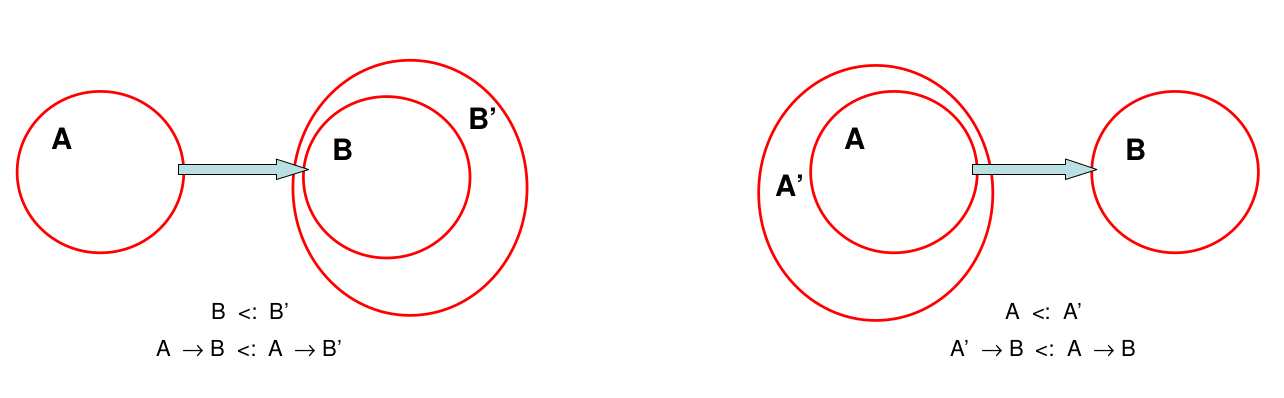
\includegraphics[scale=0.25]{img/subtipado/funciones-diagrama-perla.png}
    \caption{Esquema de Perla para entender el subtipado de funciones}
\end{figure}


\[
    \deriv{S-Arrow | S-Func}
        {\subt{\sigma'}{\sigma} \quad \subt{\tau}{\tau'}}
        {\subt
            {\tfunc{\sigma}{\tau}}
            {\tfunc{\sigma'}{\tau'}}
        }
\]

Para reemplazar una función por otra, tiene que
\begin{itemize}
    \item Bancarse todos los argumentos, o más (contravarianza)
    \item El resultado tiene que ser reemplazable (covarianza)
\end{itemize}

Se dice que el constructor de tipos de función es \textbf{contravariante} en el
primer argumento (dominio) y \textbf{variante} en el segundo (imagen).

\subsection{Subtipado de referencias}

Ref es \textbf{invariante}, solo se comparan referencias de tipos equivalentes

\[
    \deriv{S-Ref}
        {\subt{\sigma}{\tau} \quad \subt{\tau}{\sigma}}
        {\subt{\tref{\sigma}}{\tref{\tau}}}
\]

\textit{no hace falta que sean iguales, como con los registros y las permutaciones}.

\begin{nota}
    Justificación

    \textbf{Es ref covariante?}

    \[
        \deriv{S-Ref}
            {\subt{\sigma}{\tau}}
            {\subt{\tref{\sigma}}{\tref{\tau}}}
    \]

    Si tengo $r: \tref{Nat}$ y hago $\dealloc{r}$, que le puedo pasar? Y la
    escritura?

    Si fuera covariante, uno esperaría que como $\subt{Int}{Float}$,
    $\subt{\tref{Int}}{\tref{Float}}$. Pero si tengo

    \begin{verbatim}
    let r = ref 3  // r : Ref Int
    in
        r := 2.1;  // Ref Int <: Ref Float, T-Sub, r: Ref Float
        !r
        // r: Int
        // Pero 2.1 no es int!
    \end{verbatim}

    se rompe con la asignación.

    (el 2 es un int que lo puedo ver como 2.0, float, pero el 2.1 es un float y
    no lo puedo ver como int)

    \textbf{Es ref contravariante?}

    \[
        \deriv{S-Ref}
            {\subt{\sigma}{\tau}}
            {\subt{\tref{\tau}}{\tref{\sigma}}}
    \]

    Como $\subt{Int}{Float}$ y suponemos ref contravariante,
    $\subt{\tref{Float}}{\tref{Int}}$

    \begin{verbatim}
    let r = ref 2.1 // r: Ref Float
    in
        !r
        // Por Ref Float <: Ref Int y T-Sub, r: Ref Int
        // r: Int
        // Pero 2.1 no es Int!
    \end{verbatim}
\end{nota}

\subsubsection{Refinado de Ref}

Para permitir algún tipo de subtipado, se agregan nuevas clases referencias de
solo lectura y solo escritura. $\tsource{\sigma}$ de lectura y $\tsink{\sigma}$
de escritura.

\[
    \ederiv
        {\GStipa{M}{\tsource{\sigma}}}
        {\GStipa{\dealloc{M}}{\sigma}}
    \quad
    \ederiv
        {\GStipa{M}{\tsink{\sigma}} \quad \GStipa{N}{\sigma}}
        {\GStipa{\assign{M}{N}}{\tunit}}
\]

\begin{itemize}
    \item Source (lectura) es covariante
    
    \[
        \deriv{S-Source}
            {\subt{\sigma}{\tau}}
            {\subt{\tsource{\sigma}}{\tsource{\tau}}}
        \quad
        \ederiv
            {\subt{Int}{Float}}
            {\subt{\tsource{Int}}{\tsource{Float}}}
    \]

    $\dealloc{r}$ puede verse como $Float$ aunque $r$ sea de tipo
    $\tsource{Int}$.

    Si tengo un ref 3 y lo desreferencio, puedo verlo como int o float 3.0
    
    \begin{verbatim}
        let r = ref 3
        in
            !r  // por Source Int <: Source Float
        :: Float
    \end{verbatim}

    Si espero leer una ref a T, puedo esperar una ref a un tipo más bajo, más
    informativo.

    \item Sink (escritura) es contravariante.

    \[
        \deriv{S-Sink}
            {\subt{\tau}{\sigma}}
            {\subt{\tsource{\sigma}}{\tsource{\tau}}}
        \quad
        \ederiv
            {\subt{Int}{Float}}
            {\subt{\tsink{Float}}{\tsink{Int}}}
    \]

    Por ejemplo,

    \begin{verbatim}
        let r = ref 2.1
        in
            r := 3; // Usando Sink Float <: Sink Int
            !r
        :: Float
    \end{verbatim}

    Puedo coercionar 3 a 3.0 y no se rompe nada.

    Si espero escribir sobre una Ref a T, puedo esperar una Ref a un tipo más
    alto, menos informativo.
\end{itemize}

Se pueden relacionar con Ref,

\[
    \deriv{S-RefSource}
        {}
        {\subt{\tref{\tau}}{\tsource{\tau}}}
    \quad
    \deriv{S-RefSink}
        {}
        {\subt{\tref{\tau}}{\tsink{\tau}}}
\]

\subsection{Algoritmo}

Muy lindo todo, pero como lo usamos para tipar? Hasta ahora nuestras reglas eran
dirigidas por sintaxis, por lo que es inmediato implementar un algoritmo de
chequeo de tipos a partir de ellas.

Pero con T-Subs, está guiada por la \textit{oportunidad del tipo}, la podés
aplicar cuando quieras como convenga. Esto hace que \textbf{no sea evidente como
implementar un algoritmo} de chequeo de tipos a partir de las reglas, que no sea
determinístico. Nos podemos sacar de encima el problema?

Propuesta N°1 de sistema: cambio en la regla de aplicación

La única regla en la que realmente hace falta subtipar es en la
aplicación. Definimos una variante del sistema de tipado dirigida por sintaxis y
la notamos con $\mapsto$.

\newcommand{\GtipaAlt}[2]{\Gamma \mapsto #1 : #2}

\[
    \deriv{T-App}   
        {
            \GtipaAlt{M}{\tfunc{\select{\sigma}}{\tau}}
            \quad \GtipaAlt{N}{\select{\rho}}
            \quad \select{\subt{\rho}{\sigma}}
        }
        {\GtipaAlt{\app{M}{N}}{\tau}}
\]

(y cambiando el resto del sistema para que use el tipado alternativo $\mapsto$)

\begin{proposition} Se puede probar por inducción en las reglas de tipado que
    \begin{enumerate}
        \item $\GtipaAlt{M}{\sigma}$ implica que $\Gtipa{M}{\sigma}$
        \item $\Gtipa{M}{\sigma}$ implica que existe $\tau$ tal que
        $\GtipaAlt{M}{\tau}$ con $\subt{\tau}{\sigma}$.
    \end{enumerate}
\end{proposition}

Pero nos falta cubrir como implementar la relación $<:$. (recordar
\fullref{sec:subt-reglas} y S-Rcd). Las reglas S-Refl y S-Trans no están guiadas
por la sintaxis. Para sacarlas,

\begin{nota}
    Diego: Lo que sigue ahora es algo anecdótico
\end{nota}

\begin{itemize}
    \item S-Refl está para resolver cosas de la pinta $\subt{Nat}{Nat}$,
    entonces podemos remover la necesidad de la reflexividad agregando axiomas
    para cada tipo: $\subt{Nat}{Nat}$, $\subt{Float}{Float}$,
    $\subt{Bool}{Bool}$.

    \textit{Esto se puede probar en general pero no lo probamos}

    \item Con un argumento similar, se puede demostrar que no es necesaria
    S-Trans agregando todas las combinaciones.
\end{itemize}

Sacando esas dos reglas, la parte de subtipado puede ser guiada por sintaxis?
Si, el algoritmo es el siguiente

\begin{verbatim}
subtype(S, T) {
    // Si es un axioma, sabemos que si. Sino,
    // func
    if S == S1 -> S2 and T == T1 -> T2:
        return subtype(T1, S2) and subtype(S2, T2)
    
    // reg
    if S == {kj: Sj, j in 1..m} and T == {li: Ti, i in 1..n}:
        return {li, i in 1..n} subseteq {kj, j in 1..m} and
            forall i exists j kj = li and subtype(Sj, Ti)

    return false
}
\end{verbatim}

\chapter{Paradigma de objetos}

El modelo de cómputo que está detrás de POO, también puede caer diseño orientado
a objetos pero es mucho más complejo. Acá vamos a modelar una parte chiquita.

\section{Programación Orientada a Objetos}

\subsubsection{Conceptos y metáfora}

\begin{itemize}
    \item Todo programa es una simulación, y cada entidad del sistema siendo
    simulado se representa en el programa a través de un \textbf{objeto}
    \item Los objetos son la forma de abstraer un concepto físico o conceptual
    del mundo real
    \item El modelo de cómputo consiste en envío de mensajes: un sistema está
    formado por objetos que \textit{colaboran} entre sí mediante mensajes.
    \item Los \textbf{mensajes} son solicitudes para que un objeto lleve a cabo
    operación. El \textbf{receptor} (el objeto que lo recibe) decide como
    llevarla a cabo, cuya implementación está descripta por un \textbf{método}.
    \item El conjunto de mensajes que responde un objeto se denomina
    \textbf{interfaz} o \textbf{protocolo}.
    \item Los objetos pueden tener \textbf{estado} interno que altere el
    comportamiento de los métodos. Se representa a través de un conjunto de
    \textbf{colaboradores internos} (también llamados \textbf{atributos} o
    \textbf{variables instancia})
\end{itemize}

Ejemplo:

\begin{verbatim}
unRectangulo
    interfaz: area
    atributos: alto y ancho
    método: area = function() { return alto * ancho }
\end{verbatim}

La única manera de interactuar con un objeto es a través de su protocolo. Su
implementación no puede depender de detalles de implementación de otros objetos
(principio heredado de TADs)

\begin{definition*}[Principio de ocultamiento de la información]
    El estado de un objeto es \textbf{privado} y solamente puede ser consultado
    o modificado por sus métodos. \textit{(No todos los lenguajes imponen esta
    restricción)}
\end{definition*}

\subsection{Method dispatch}

Cómo hacemos por atrás para saber qué método de un objeto ejecutar cuando le
llega un mensaje? El proceso que establece la asociación mensaje-método a
ejecutar se llama \textbf{method dispatch}.

Si se hace en tiempo de \textit{compilación} (se puede determinar a partir del
código fuente) es \textbf{method dispatch estático}. En cambio, si se hace en
runtime es \textbf{method dispatch dinámico.}

\subsection{Corrientes}

Quien es responsabile de conocer los métodos de los objetos? Hay dos
alternativas conocidas: \textbf{clasificación} y \textbf{prototipado}

\subsection{Clasificación}

Es la más mainstream. Las clases modelan \textbf{conceptos abstractos} del
dominio de problema. Definen el comportamiento y la forma de un conjunto de
objetos que instancian (sus \textbf{instancias}). Todo objeto es instancia de
alguna clase. Son templates que tienen métodos, atributos y después se usan para
instanciar objetos concretos.

Tienen

\begin{itemize}
    \item Nombre
    \item Definición de variables de instancia
    \item Métodos de instancia. Por cada uno nombre, parámetros y cuerpo.
\end{itemize}

\begin{figure}[H]
    \centering
    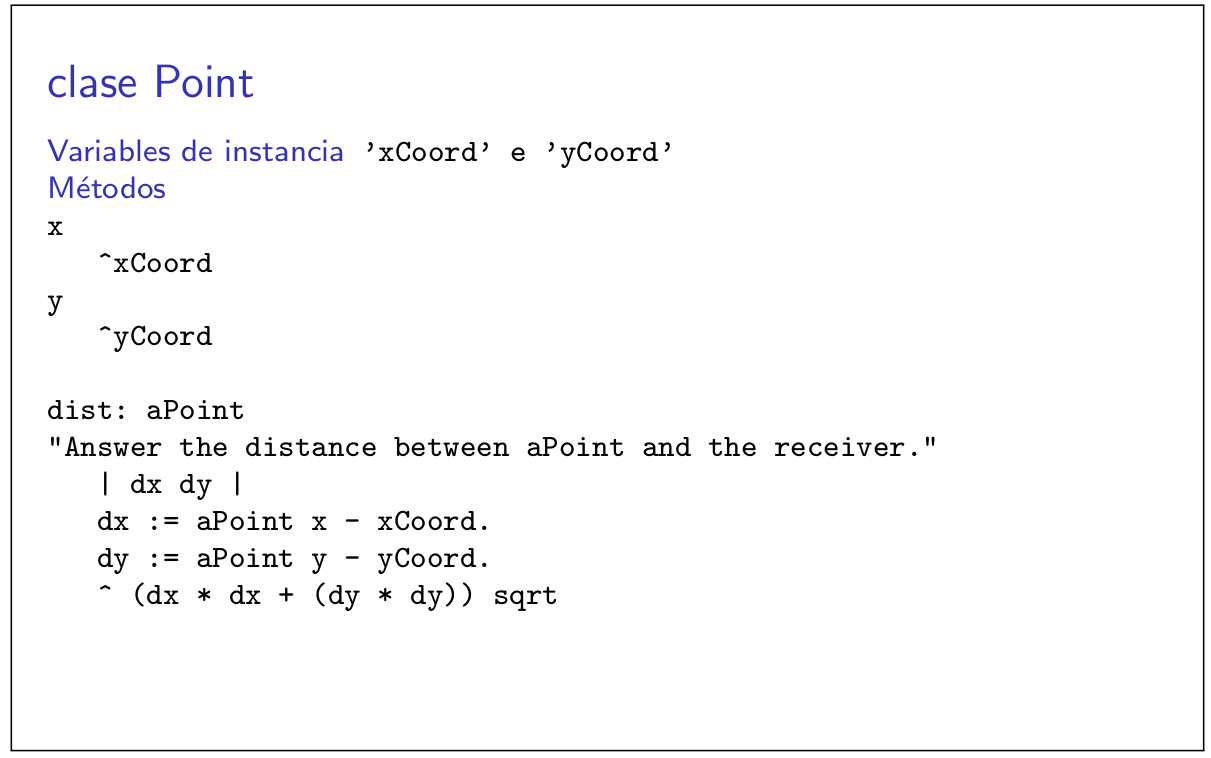
\includegraphics[scale=0.25]{img/poo/st-point.png}
    \caption{Ejemplo de clase en sintaxis de Smalltalk}
\end{figure}

\begin{figure}[H]
    \centering
    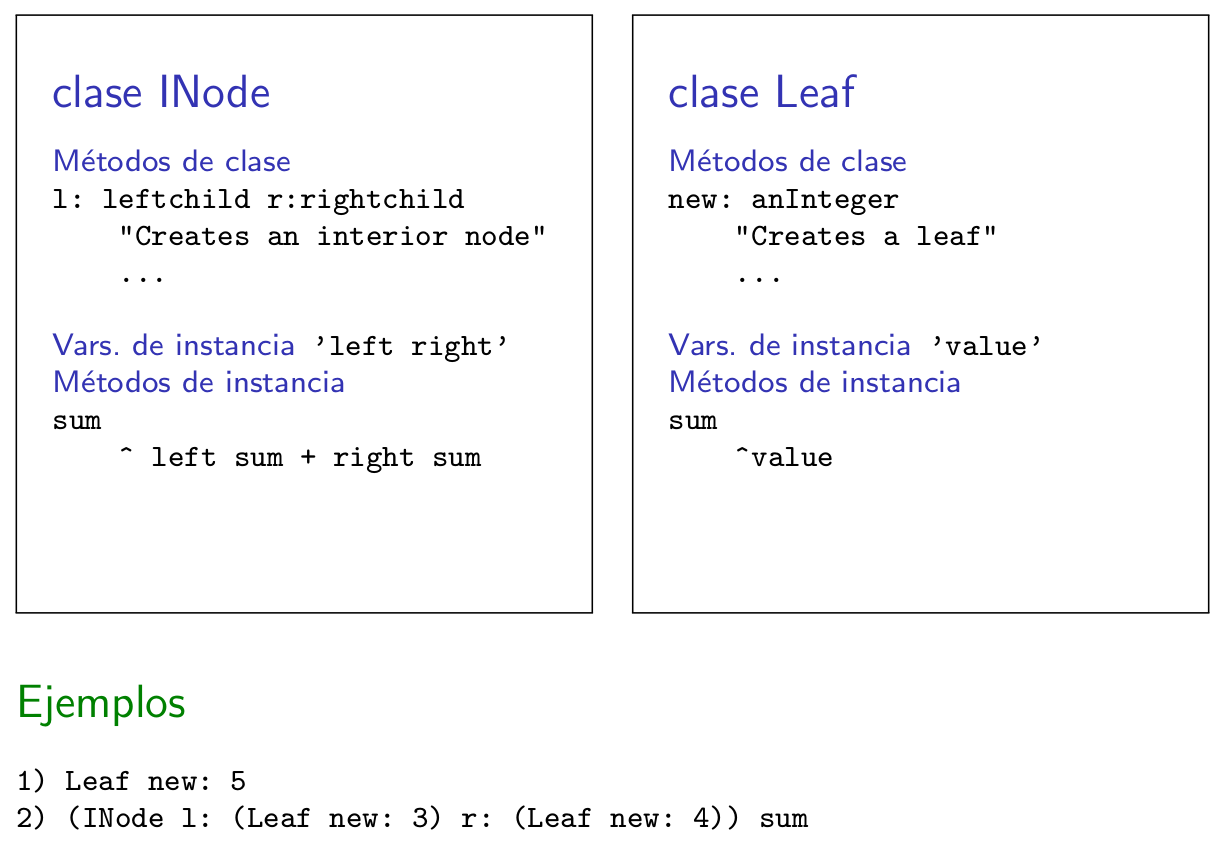
\includegraphics[scale=0.25]{img/poo/st-node.png}
    \caption{Ejemplo de clase Node en sintaxis de Smalltalk}
\end{figure}

\subsubsection{Self y super}

\textbf{self} es una pseudovariable que durante la ejecución de un
método referencia al receptor del mensaje. Se liga automáticamente y no puede
ser asignada.

\begin{figure}[H]
    \centering
    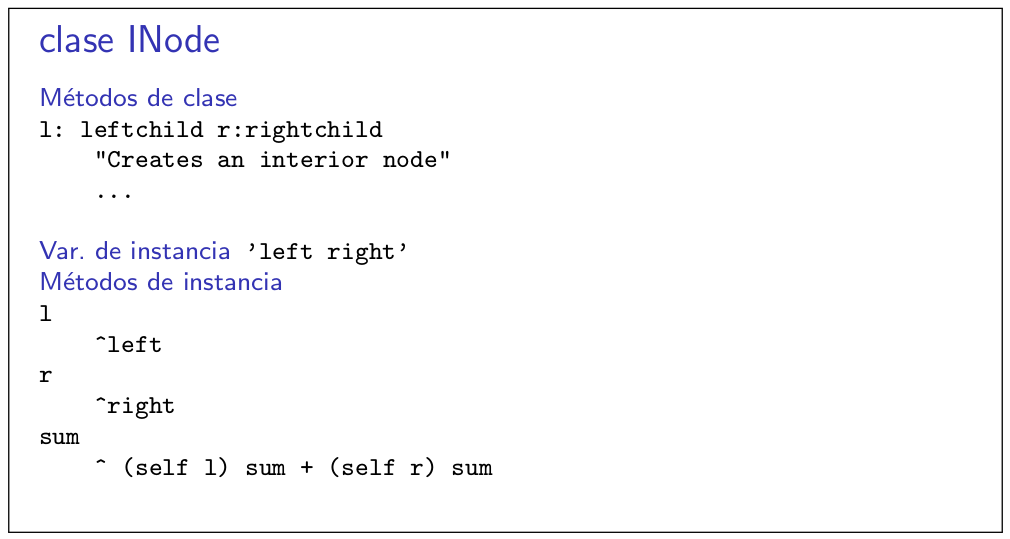
\includegraphics[scale=0.25]{img/poo/st-self.png}
    \caption{Ejemplo uso de self en Smalltalk}
\end{figure}

\textbf{super} es otra pseudovariable que referencia al objeto que recibe el
mensaje. Cambia el proceso de activación al momento del envío de un mensaje.

Una expresión de la forma \texttt{super msg} que aparece en el cuerpo de un
método \texttt{m} provoca que el \textbf{method lookup} se haga desde el padre
de la clase anfitriona de \texttt{m}.

\begin{figure}[H]
    \centering
    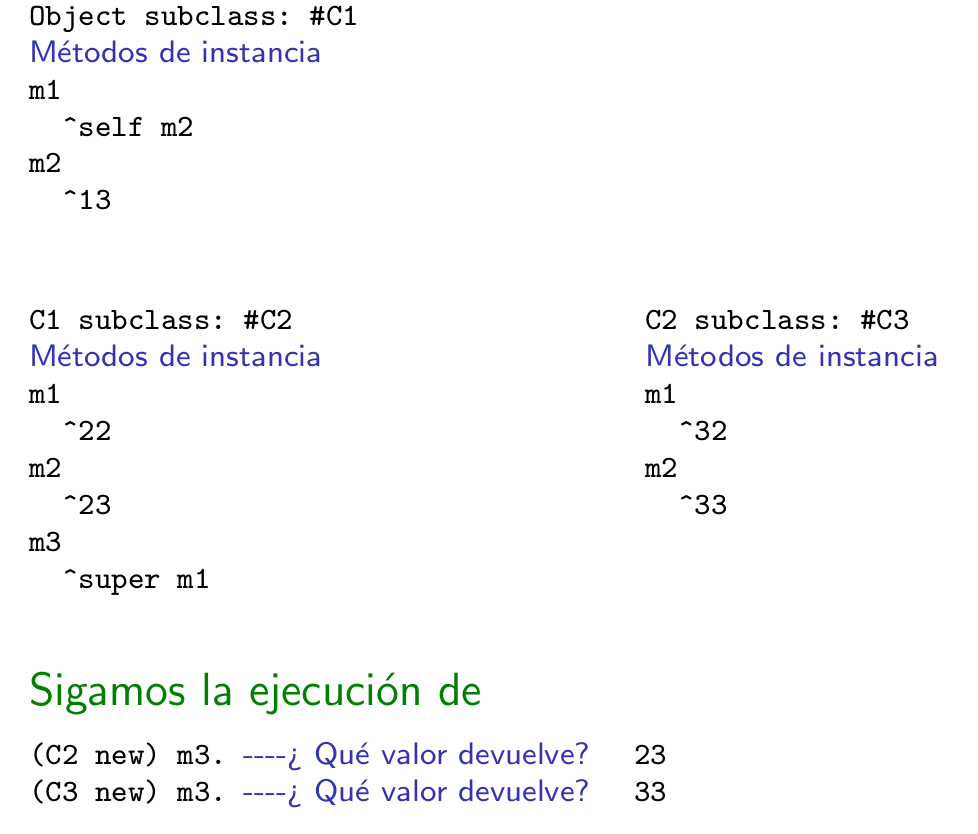
\includegraphics[scale=0.25]{img/poo/st-super-self.png}
    \caption{Ejemplo \texttt{super} y \texttt{self}}
\end{figure}

\subsubsection{Jerarquía de clases}

Es común que nuevas clases se definan como \textit{extensiones} de clases
existentes, agregando o cambiando el comportamiento de algunos métodos y
agregando nuevas variables de instancia o clase. Por eso, una clase puede
\textbf{heredar de} o \textbf{extender} de una clase existente (llamada
\textbf{superclase}). La transitividad de esta relación induce nociones de
\textbf{ancestros} y \textbf{descendientes}.

Hay dos tipos

\begin{itemize}
    \item \textbf{Simple}: una clase tiene un único padre (salvo la raíz). Esta
    es la que usan la mayoría de los lenguajes OO.
    \item \textbf{Múltiple}: una clase puede tener más de una clase padre.
    
    Complica el proceso de method dispatch, ya que si tengo un método $m$
    definido en más de una superclase, cual uso? Hay dos soluciones posibles:
    \begin{itemize}
        \item Establecer un \textit{orden de búsqueda} sobre las superclases
        \item Pedir que se \textit{redefinan} en la clase nueva todos los
        métodos que estén en más de una clase padre.
    \end{itemize}
    
\end{itemize}

\begin{figure}[H]
    \centering
    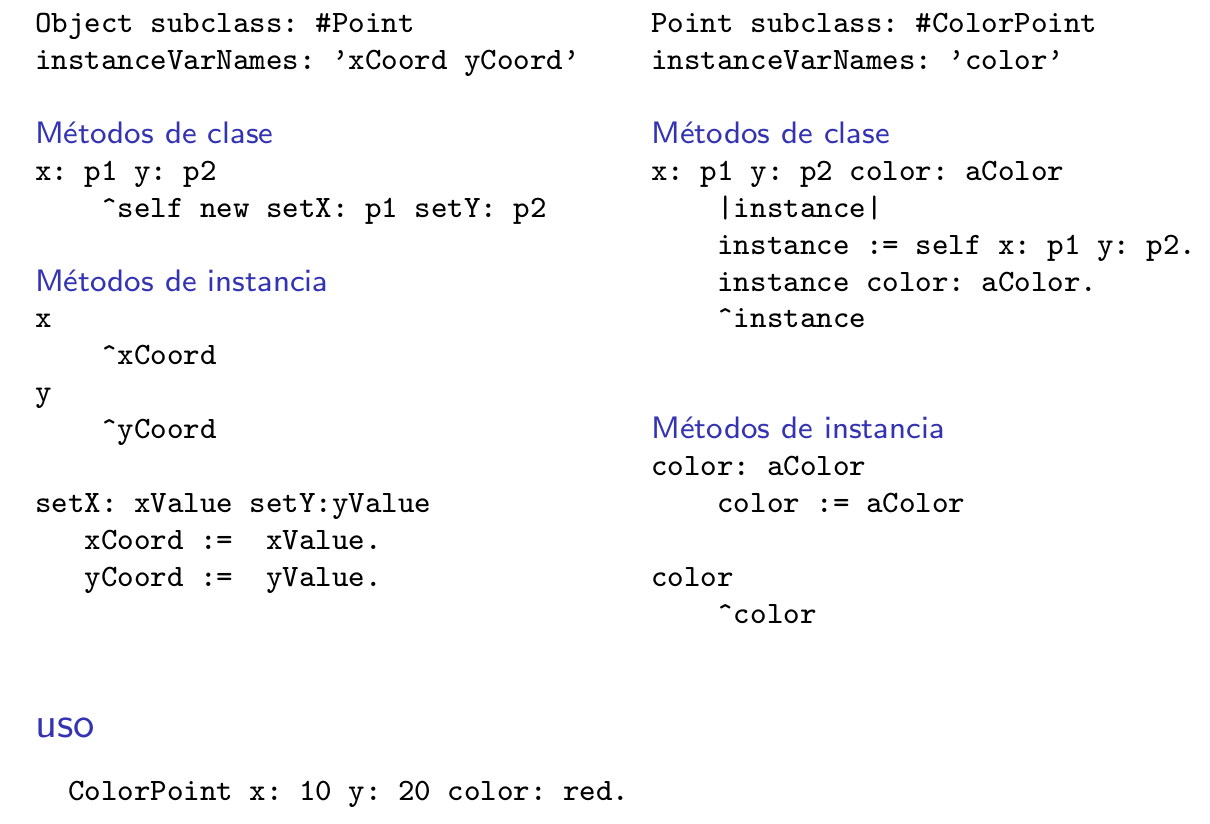
\includegraphics[scale=0.25]{img/poo/st-inheritance.png}
    \caption{Ejemplo de herencia en Smalltalk}
\end{figure}

\subsection{Prototipado}

Construye instancias concretas que se interpretan como representantes canónicos
de instancias (llamados prototipos). El resto de las instancias se generan
clonando los prototipos (de forma shallow). Y los clones se pueden cambiar.

Ejemplo de creado de objeto en js

\begin{minted}{javascript}
let celda = {
    contenido: 0,
    get: function() { return this.contenido; },
    set: function(n) { this.contenido = n; }
}

// Generar objetos
Celda = function() {
    this.contenido = 0;
    this.get = function() { return this.contenido; };
    this.set = function(n) { this.contenido = n; };
}

otracelda = new Celda();
\end{minted}

\newcommand{\obj}[1]{[\ #1\ ]} % objeto
\newcommand{\attr}[2]{#1 = #2} % atributo
\newcommand{\met}[2]{\varsigma (#1) #2} % method{args}{body}
\newcommand{\sel}[2]{#1.#2} % selección o envío de mensaje
\newcommand{\update}[3]{\sel{#1}{#2} \Leftarrow #3} % redefinición de método (update)
% TODO: Debería ser algún harpoon pero no encontré como hacerlo
\newcommand{\asgn}[3]{\sel{#1}{#2} := #3}

\newcommand{\sfv}[1]{\text{fv}(#1)}
\newcommand{\ssust}[3]{#1 \select{\{#2 / #3\}}} % sigma sust

\newcommand{\attrLi}{\attr{l_i}{\met{x_i}{\iesimo{b}}}}

\newcommand{\sderiv}[3]{\trfrac[{[}#1{]}]{#2}{#3}}
\newcommand{\bigreduces}{\longrightarrow}
\newcommand{\bigreduce}[2]{#1 \bigreduces #2}

\section{Cálculo de objetos}

Acá vamos a hacer semántica big step en vez de small step. De un gran paso
llegás al valor. Vamos a ver un cálculo de objetos no tipado basado en Abadi y
Cardelli, 98 que se llama $\varsigma$ calculo (sigma pero una sigma cheta)

Ingredientes

\begin{itemize}
    \item Los objetos son la única estructura computacional
    \item Los objetos son registros que tienen métodos como atributos (un campo
    normal va a ser un método que devuelve siempre lo mismo)
    \item Cada método tiene una única variable ligada que representa a
    \texttt{self} (o \texttt{this}) y un cuerpo que produce el resultado, que
    puede depender o no de self.
    \item Proveen dos operaciones: envío de mensaje (invocar un método) o
    redefinición de un método.
\end{itemize}

\subsection{Sintaxis}

\begin{alignat*}{3}
    o, b ::=
    &  &&x  &&\text{\textit{variable}}\\
    &|\ &&\obj{\attr{l_i}{\met{x_i}{\iesimo{b}}}} 
    \quad&&\text{\textit{objeto}}\\
    &| &&\sel{o}{l} &&\text{\textit{selección / envío de mensaje}}\\
    &| &&\update{o}{l}{\met{x}{b}} &&\text{\textit{redefinición de método}}\\
\end{alignat*}

\begin{example*}
    \[
    o \eqdef \obj{
        \attr{l_1}{\met{x_1}{\obj{}}},\
        \attr{l_2}{\met{x_2}{\sel{x_2}{l_1}}}
    }
    \]

    \begin{itemize}
        \item $l_1$ retorna el objeto vacío
        \item $l_2$ envía el mensaje $l_1$ a self (representado por el parámetro $x_2$)
    \end{itemize}
\end{example*}

\subsection{Atributos vs métodos}

El cálculo $\varsigma$ no incluye explícitamente atributos (campos), sino que se
representan como métodos que no usan al parámetro self. De esta manera, el envío
de un mensaje representa también a la selección de un atributo y la redefinición
de un método representa también la asignación de un atributo

Como abusos de notación, vamos a

\begin{itemize}
    \item Usar $\obj{\dots, \attr{l}{b}, \dots}$ en vez de
    $\attr{l}{\met{x}{b}}$ cuando no se usa $x$ en $b$,
    \item Usar $\asgn{o}{l}{b}$ en vez de $\update{o}{l}{\met{x}{b}}$ cuando $x$
    no se usa en $b$.
\end{itemize}

\subsection{Variables libres}

$\varsigma$ es un ligador del parámetro self $x_i$ en el cuerpo $b_i$ de la
expresión $\met{x_i}{b_i}$.

\begin{nota}
    Esto es similar a lc, probablemente en semántica vamos a tener que hacer una
    sustitución para ligarla.
\end{nota}

\begin{definition}[Variables libres]
\begin{alignat*}{2}
    &\sfv{\met{x}{b}} &&= \sfv{b} \setminus \{ x \}\\
    &\sfv{x} &&= \{ x \} \\
    &\sfv{\obj{\attrLi}}
        &&= \bigcup_{i\in 1..n} \sfv{\met{x_i}{b_i}}\\
    &\sfv{\sel{o}{l}} &&= \sfv{o} \\
    &\sfv{\update{o}{l}{\met{x}{b}}} &&= \sfv{o.l} \cup \sfv{\met{x}{b}}
\end{alignat*}

Un término $o$ es \textbf{cerrado} si $\sfv{o} = \emptyset$.
\end{definition}

\subsection{Sustitución}

\begin{alignat*}{2}
    &\ssust{x}{c}{x} &&= c \\
    &\ssust{y}{c}{x} &&= y \\
    &\ssust{(\obj{\attrLi})}{c}{x}
    &&= \obj{
        \attr
            {l_i}
            {\ssust{(\met{x_i}{b_i})}{c}{x}^{i\in 1..n}}
    }\\
    &\ssust{(\sel{o}{l})}{c}{x} &&= \sel{\ssust{o}{x}{x}}{l}\\
    &\ssust{\update{o}{l}{\met{y}{b}}}{c}{x}
        &&= \update{(\ssust{o}{c}{x})}{l}{(\ssust{(\met{y}{b})}{c}{x})}\\
    &\ssust{(\met{y}{b})}{c}{x} &&=
        \met{y'}{\ssust{\ssust{b}{y'}{y}}{c}{x}}\\
    & && \qquad \text{con } y' \notin
        \sfv{\met{y}{b}}
        \cup \sfv{c}
        \cup \{ x \}
\end{alignat*}

Acomodamos las cosas para que no haya interferencias en la sustitución como
clashing de nombres (primer reemplazo) y una vez que tengamos eso, aplicamos la
sustitución que queremos.

\subsection{Equivalencia de términos ($\equiv$)}

Los términos $\met{x}{b}$ y $\met{y}{(\ssust{b}{y}{x})}$ con $y \notin
\sfv{b}$ se consideran equivalentes ($\alpha$-conversión).

También, dos objetos que difieren en el orden de sus componentes son
considerados equivalentes.

\[
    \obj{
        \attr{l_1}{\met{x_1}{\obj{}}},\
        \attr{l_2}{\met{x_2}{\sel{x_2}{l_1}}}
    }
    \equiv
    \obj{
        \attr{l_2}{\met{x_3}{\sel{x_3}{l_1}}},\
        \attr{l_1}{\met{x_1}{\obj{}}}
    }
\]

\subsection{Semántica operacional}

\begin{nota}
    En lc, las reducciones llevaban de $\reduce{M}{M'}$ y eventualmente
    aplicando muchas reducciones llegábamos a un valor. Acá vamos a llegar en
    una sola.
\end{nota}

Los valores van a ser objetos

\[
    v ::= \obj{\attrLi}
\]

Y vamos a aplicar reducciones \textbf{big-step} $\bigreduces$, que en un paso de reducción
pasan de una expresión a un valor.
\begin{gather*}
    \sderiv{Obj}{}{\bigreduce{v}{v}}\\
    \sderiv{Sel}
        {
            \bigreduce{o}{v'}
            \quad v' \equiv \obj{\attrLi}
            \quad \bigreduce{\ssust{b_j}{v'}{x_j}}{v}
            \quad j\in 1..n
        }
        {\bigreduce{\sel{o}{l_j}}{v}}\\
    \sderiv{Upd}
        {
            \bigreduce{o}{\obj{\attrLi}}
            \quad j \in 1..n
        }
        {
            \bigreduce
                {\update{o}{l_j}{\met{x}{b}}}
                {\obj{
                    \attr{l_j}{\met{x}{b}},\
                    \attr{l_i}{
                        \met{x_i}{b_i}^{i\in1..n-\{j\}}
                    }
                }}
        }
\end{gather*}

En Sel reduzco $o$ hasta un valor $v'$ para saber quien es self, ligo self en
$b_j$ que es el cuerpo del método correspondiente a $l_j$, y el resultado es
reducir eso a un valor

\end{document}

